\documentclass[a4paper]{article}
\usepackage[spanish]{babel}
\usepackage[utf8]{inputenc}
\usepackage{charter}   % tipografia
\usepackage{graphicx}
\usepackage{algorithmic}
\usepackage{amsmath}
%\usepackage{algorithm}
%\usepackage[noend]{algpseudocode}

\usepackage[bookmarks = true, colorlinks=true, linkcolor = black, citecolor = black, menucolor = black, urlcolor = blue]{hyperref} 


%\usepackage{makeidx}
\usepackage{paralist} %itemize inline
\usepackage[ruled,vlined]{algorithm2e}
\usepackage{float}
\usepackage{caption}
%\usepackage{amsmath, amsthm, amssymb}
%\usepackage{amsfonts}
%\usepackage{sectsty}
%\usepackage{charter}
%\usepackage{wrapfig}
\usepackage{listings}
\usepackage[svgnames, table, usenames, dvipsnames]{xcolor}

\definecolor{mygreen}{rgb}{0,0.6,0}
\definecolor{mygray}{gray}{0.25}
\definecolor{myblue}{rgb}{0.2,0.2,0.6}

%Estilos para el c\'odigo fuente
\lstset{
	basicstyle=\ttfamily\scriptsize,
	breaklines=true,
	captionpos=b,
	commentstyle=\color{mygreen},
	escapechar=@,
	extendedchars=true,
	identifierstyle=\color{myblue},
	language=java,
	numbers=left,
	numberstyle=\tiny\color{mygray},
	stringstyle=\color{orange},	
	tabsize=3
}


\usepackage{color} % para snipets de codigo coloreados
\usepackage{fancybox}  % para el sbox de los snipets de codigo

\definecolor{litegrey}{gray}{0.94}

% \newenvironment{sidebar}{%
% 	\begin{Sbox}\begin{minipage}{.85\textwidth}}%
% 	{\end{minipage}\end{Sbox}%
% 		\begin{center}\setlength{\fboxsep}{6pt}%
% 		\shadowbox{\TheSbox}\end{center}}
% \newenvironment{warning}{%
% 	\begin{Sbox}\begin{minipage}{.85\textwidth}\sffamily\lite\small\RaggedRight}%
% 	{\end{minipage}\end{Sbox}%
% 		\begin{center}\setlength{\fboxsep}{6pt}%
% 		\colorbox{litegrey}{\TheSbox}\end{center}}

\newenvironment{codesnippet}{%
	\begin{Sbox}\begin{minipage}{\textwidth}\sffamily\small}%
	{\end{minipage}\end{Sbox}%
		\begin{center}%
		\vspace{-0.4cm}\colorbox{litegrey}{\TheSbox}\end{center}\vspace{0.3cm}}



\usepackage{fancyhdr}
\pagestyle{fancy}

%\renewcommand{\chaptermark}[1]{\markboth{#1}{}}
\renewcommand{\sectionmark}[1]{\markright{\thesection\ - #1}}

\fancyhf{}

\fancyhead[LO]{Sección \rightmark} % \thesection\ 
\fancyfoot[LO]{\small{}}
\fancyfoot[RO]{\thepage}
\renewcommand{\headrulewidth}{0.5pt}
\renewcommand{\footrulewidth}{0.5pt}
\setlength{\hoffset}{-0.8in}
\setlength{\textwidth}{16cm}
%\setlength{\hoffset}{-1.1cm}
%\setlength{\textwidth}{16cm}
\setlength{\headsep}{0.5cm}
\setlength{\textheight}{25cm}
\setlength{\voffset}{-0.7in}
\setlength{\headwidth}{\textwidth}
\setlength{\headheight}{13.1pt}

\renewcommand{\baselinestretch}{1.1}  % line spacing


\usepackage{underscore}
\usepackage{caratula}
\usepackage{hyperref}
%\usepackage{tikz}
\usepackage{enumitem}

\newlength{\wideitemsep}
\setlength{\wideitemsep}{.7\itemsep}
\addtolength{\wideitemsep}{-3pt}
%\let\olditem\item
%\renewcommand{\item}{\setlength{\itemsep}{\wideitemsep}\olditem}

\let\olditemize\itemize
\def\itemize{\olditemize\itemsep=10pt }

\begin{document}

\thispagestyle{empty}
\materia{Algoritmos y Estructuras de Datos III}
\submateria{Segundo Cuatrimestre de 2015}
\titulo{Trabajo Práctico III}
%\subtitulo{subtitulo del trabajo}
\integrante{Bouzón, María Belén}{128/13}{belenbouzon@hotmail.com}
\integrante{Jiménez, Paula}{655/10}{puly05@gmail.com}
\integrante{Montepagano, Pablo}{205/12}{pablo@montepagano.com.ar}
\integrante{Rey, Maximiliano}{037/13}{rey.maximiliano@gmail.com}


\maketitle
\newpage

\thispagestyle{empty}


\thispagestyle{empty}
\vspace{3cm}
\tableofcontents
\newpage

\newpage
\section{Problema 1: Algoritmo Exacto para 2-List Coloring}

\subsection{Descripción de la problemática}
Este ejericicio está centrado en la resolución de un problema particular de coloreo, 2-listColoring. En este caso, cada nodo se puede colorear solo con uno o dos colores específicos. El algoritmo debe determinar si existe o no un coloreo en donde no existen dos nodos consecutivos del mismo color y, en caso afirmativo, encontrar una solución.
Este problema es facilmente reducible a 2-SAT, por lo cual existen algortmos polinomiales que lo resuelven.

\subsection{Resolución propuesta y justificación}
Como mencionamos antes, el problema del 2-ListColoring es fácilmente reducible a un problema de 2-SAT, y en esto se basa el algoritmo implementado. Si existe una coloración posible, entonces el hecho de que un determinado nodo esté pintado de un color implica que ninguno de sus vecinos esta pintado del mismo. Además, si un nodo tiene dos colores posibles, el nodo esta pintado de un color C1 si y solo si no esta pintado del color C2.
El 2-SAT se representa con un grafo dirigido en donde un nodo A (que representa una proposición) apunta a un nodo B si A implica B.

Sean x, y, z proposiciones representadas por nodos de nuestro grafo dirigido, si en el grafo existe una arista desde el nodo que representa a x al nodo que representa a y, y otra arista entre el nodo que representa a y al nodo que representa a z, esto significa que x $\rightarrow$ y e y $\rightarrow$ z, de lo cual se deduce que x $\rightarrow$ z. Generalizando se puede decir que, dadas x, z proposiciones,  x $\rightarrow$ z si y solo si existe un camino desde el nodo que representa a x hasta el nodo que representa a z. Es decir, en este contexto una componente fuertemente conexa representa un conjunto de proposiciones de las cuales se puede afirmar que todas son válidas o todas son falsas. 

Para la resolución del 2-SAT, se implementa el algoritmo de Kosaraju. Este algoritmo recibe como entrada un grafo dirigido y devuelve como resultado las componentes fuertemente conexas que se encuentran en el mismo. 

Como el algoritmo de Kosaraju encuentra todas las componentes fuertemente conexas, entonces, dadas dos componentes C1 y C2, si existe un camino entre C1 y C2, no puede existir un camino desde C2 a C1 (de lo contrario ambas debería estar en la misma componente). Además, si existe un camino entre C1 y C2, con el algoritmo de Kosaraju C1 será detectada antes que C2. Nuestra implementación fue diseñada para que la lista de componentes fuertemente conexas resultante del algoritmo preserve este orden de detección. Posteriormente de la ejecución del Kosaraju, nuestro algoritmo registra, para cada componente conexa, cual es la componente conexa que contiene la negación de sus proposiciones. En caso de que una misma componente conexa contenga a una proposición y su negación, entonces se determina que el problema no tiene solución, ya que implicaría que, sea x la proposición en cuestión, x $\leftrightarrow$ $\lnot$x.

Finalmente comienzan a fijarse los valores de verdad, recorriendo las componentes fuertemente conexas en el orden en que fueron obtenidas en el paso anterior. Si a la componente aún no se le asignó un valor de verdad, se le asigna false. Cuando se fija un valor para una componente determinada, a la componente que contiene la negación de sus proposiciones se le asigna el valor opuesto.  Además, si a una componente se le asigna false, todos las componentes que implican a la misma (es decir, todas las componentes desde las cuales existe un camino hasta la componente evaluada) también se les asigna false (recursivamente). Y, si a una componente se le asigna true, a todas las componentes que son implicadas por la misma se  les asigna también true. Si el algoritmo encuentra una contradicción (es decir, una componente que a la que se busca  asignar false ya tiene true o viceversa), determina que el problema no tiene solución.

Una vez determinados los valores de verdad, se deduce la coloración de los nodos del grafo original a partir de las proposiciones que forman parte de las componentes evaluadas como verdaderas.

\begin{algorithmic} 
\newcommand{\INDSTATE}[1][1]{\STATE\hspace{#1\algorithmicindent}}
 \STATE{Algoritmo2ListColoring(grafo_original)}
	\INDSTATE[2]{GrafoDirigido = crearGrafoDirigidoConProposiciones(grafo_original)}
	\INDSTATE[2]{ListaComponentesConexas =  Kosaraju(GrafoDirigido)}
	\INDSTATE[2]{GrafoCompacto = generarGrafoCompacto(ListaComponentesConexas)
	\INDSTATE[4]{Si GrafoCompacto es INVALIDO}
		\INDSTATE[6]{Devolver NO_HAY_SOLUCION}

	\INDSTATE[4]{asignacionDeVerdad = AsignarValoresDeVerdad(ListaComponentesConexas,GrafoCompacto)}
	\INDSTATE[4]{Si asignacionDeVerdad==INVALIDO}
		\INDSTATE[6]{Devolver NO_HAY_SOLUCION}

	\INDSTATE[4]{Devolver ObtenerColoreoParaGrafoOriginal(ListaComponentesConexas)}
 \STATE Fin
\end{algorithmic} 

\begin{algorithmic}
\newcommand{\INDSTATE}[1][1]{\STATE\hspace{#1\algorithmicindent}}
\STATE crearGrafoDirigidoConProposiciones (grafo_original)
	\INDSTATE[2]{GrafoDirigido = vacio}
	\INDSTATE[2]{Para cada nodo del grafo_original}
		\INDSTATE[4]{Si cantidad_colores(nodo)==1}
			\INDSTATE[6]{GrafoDirigido.agregar(¬Acl -> Acl)}
		\INDSTATE[4]{Sino}
			\INDSTATE[6]{GrafoDirigido.agregar(Acl1 <-> ¬Acl2)}
			\INDSTATE[6]{GrafoDirigido.agregar(Acl2 <-> ¬Acl1)}
\STATE
	\INDSTATE[2]{Para cada arista (A,B)}
		\INDSTATE[4]{Para cada color comun c entre A y B}
			\INDSTATE[6]{GrafoDirigido.agregar(Ac -> ¬Bc)}
			\INDSTATE[6]{GrafoDirigido.agregar(Bc -> ¬Ac)}

	Devolver GrafoDirigido
\STATE Fin
\end{algorithmic} 

\begin{algorithmic}
\newcommand{\INDSTATE}[1][1]{\STATE\hspace{#1\algorithmicindent}}
\STATE Kosaraju(grafoDirigido)
	\INDSTATE[2]{ListaComponentesConexas = vacio}
	\INDSTATE[2]{Pila = vacio}
	\INDSTATE[2]{Para cada nodo A de grafoDirigido}
		\INDSTATE[4]{si (Pila.no_contiene(A))}
			\INDSTATE[6]{apilar nodos partiendo de A utilizando BFS}
		
	\INDSTATE[2]{grafoDirigidoInverso = grafoDirigido.invertir_aristas()}

	\INDSTATE[2]{Mientras Pila no vacia}
		\INDSTATE[4]{A = Pila.SacarPrimero}
		\INDSTATE[4]{Si (no_marcada(A))}
			\INDSTATE[6]{Componente = vacio}
			\INDSTATE[6]{agregar a Componente todos los nodos partiendo de A utilizando BFS en grafoDirigidoInverso}
			\INDSTATE[6]{marcar(A)}
			\INDSTATE[6]{ListaComponentesConexas.agrefarAlFinal(Componente)}
\STATE
	\INDSTATE[2]{Devolver ListaComponentesConexas}
\STATE Fin
\end{algorithmic}

\begin{algorithmic}
\newcommand{\INDSTATE}[1][1]{\STATE\hspace{#1\algorithmicindent}}
\STATE generarGrafoCompacto(ListaComponentesConexas)
	\INDSTATE[2]{GrafoCompacto = vacio}
	\INDSTATE[2]{Para cada componente en ListaComponentesConexas}
		\INDSTATE[4]{Para cada nodo A de componente}
			\INDSTATE[6]{Para cada arista (A,B)}
				\INDSTATE[8]{componente.agregarArista(componenteDe(B))}
			\INDSTATE[6]{Para cada nodo B negado por A}
				\INDSTATE[8]{componente.asociarComoNegacion(componenteDe(B))}
				\INDSTATE[8]{componenteDe(B).asociarComoNegacion(componente)}

				\INDSTATE[8]{Si componente==componenteDe(B)}
					\INDSTATE[10]{Devolver INVALIDO}

\STATE
	\INDSTATE[2]{Devolver GrafoCompacto}
\STATE Fin
\end{algorithmic}

\begin{algorithmic}
\newcommand{\INDSTATE}[1][1]{\STATE\hspace{#1\algorithmicindent}}
\STATE AsignarValoresDeVerdad(ListaComponentesConexas,GrafoCompacto)
	\INDSTATE[2]{Para cada componente ListaComponentesConexas}
		\INDSTATE[4]{Si no esta marcada componente}
			\INDSTATE[6]{marcar(componente,false)}
			\INDSTATE[6]{propagar false a todas las componentes que poseen un camino hasta esta componente en GrafoCompacto}
			\INDSTATE[6]{Si inconsistencia al propagar}
				\INDSTATE[8]{Devolver INVALIDO}

			\INDSTATE[6]{marcar(componente.negacionAsociada,true)}
			\INDSTATE[6]{propagar true a todas las componentes accesibles desde componente.negacionAsociada en GrafoCompacto}
			\INDSTATE[6]{Si inconsistencia al propagar}
				\INDSTATE[8]{Devolver INVALIDO}
\STATE
	\INDSTATE[2]{Devolver VALIDO}

\STATE Fin
\end{algorithmic}

\begin{algorithmic}
\newcommand{\INDSTATE}[1][1]{\STATE\hspace{#1\algorithmicindent}}
\STATE ObtenerColoreoParaGrafoOriginal(ListaComponentesConexas)
	\INDSTATE[2]{Colores = vacio}
	\INDSTATE[2]{Para cada componente con valor true en ListaComponentesConexas}
		\INDSTATE[4]{Para cada nodo con proposicion afirmativa de componente}
			\INDSTATE[6]{Colores.asignar_color(nodo.nodoDeGrafoOriginal.identidad,nodo.colorPropuesto)}
	\INDSTATE[2]{Devolver Colores}
\STATE Fin
\end{algorithmic}


\subsection{Análisis de la complejidad}
El grafo dirigido contiene a los sumo cuatro veces más nodos que el grafo de entrada, y el grafo compacto tiene a los sumo tantos nodos como el grafo dirigido. Por lo tanto, podemos afirmar que, sea n la cantidad de nodos inicial, n' la cantidad de nodos del grafo dirigido y n'' la cantidad de nodos del grafo compacto, $\mathcal{O}(f(n)) = \mathcal{O}(f(n')) = \mathcal{O}(f(n''))$ (si no se conocen datos adicionales para la entrada).

Generar el grafo dirigido a partir del grafo de entrada tiene una complejidad de $\mathcal{O}(n^2\log{n})$, ya que para cada nodo del grafo, es necesario crear los nodos dirigidos que lo representan y definir sus aristas con otros nodos. A medida que se van creando, los nodos se guardan y se buscan en un TreeSet.

El algoritmo utilizado para encontrar las componentes fuertemente conexas no recorre más de dos veces todos los nodos, por lo cual su complejidad es lineal, al igual que el algoritmo que determina el valor de verdad de los nodos compactos.

\subsection{Experimentación}
Casos de test:
\subsubsection{El triángulo}
En este test existen tres nodos interconextados en donde cada nodo comparte un color con uno de sus vecinos. El algoritmo debería encontrar la única solución posible.
Posteriormente, se le añade al triangulo un nodo extra vecino del primero con el color con el cual estaba pintado el primero, con lo cual no existe solución.
\subsubsection{El pentagono}
En esta oportunidad, se dibuja un k5. Cada nodo tiene como opción un color que no se repite en sus compañeros y otro que es compartido por más de uno. El algoritmo debería encontrar una solución
\subsubsection{El señor de los anillos}
En este caso se prueba un ciclo de seis nodos. A los pares se les asigna 0 y a los impares uno, y además todos poseen un segundo color que comparten con uno de sus vecinos. Como el grafo es bipartito, el algoritmo debería hallar una solución.
\subsubsection{Grafos bipartitos completos}
Otro de los casos se basa en generar grafos bipartitos completos. En este caso, se les asigna a todos los nodos 0 y 1. Como un grafo bipartito (en particular, uno completo) puede colorearse con dos colores, el algoritmo deberia encontrar una solución para el mismo. Posteriormente, se le añade al grafico una arista que une dos nodos que no estaban conectados, con lo que el grafo deja de ser bipartito y se necesitan 3 colores para colorearlo. En este caso, el algoritmo debería determinar que no existe solución.

\subsubsection{Testeos de complejidad}
Para testear la complejidad, se generan grafos al azar en donde todos los nodos poseen como opciones de coloreo a un color que no se repite en los demás nodos y otro que es seleccionado al azar. En una de las estrrategias se deja fija la cantidad de aristas, en otra se fija la cantidad de nodos, y en la otro se incrementan las aristas y los nodos en igual proporción.

\subsubsection{Complejidad en grafos completos}
En un último caso se generan grafos completos en donde se a incrementando la cantidad de nodos (y, logicamente, de aristas). Debido al consumo de memoria, este último caso se ha testeado con valores inferiores que al resto de los test.

% \subsubsection{Constrastación Empírica de la complejidad}


% \begin{figure}[H]
% 	\centering
%  	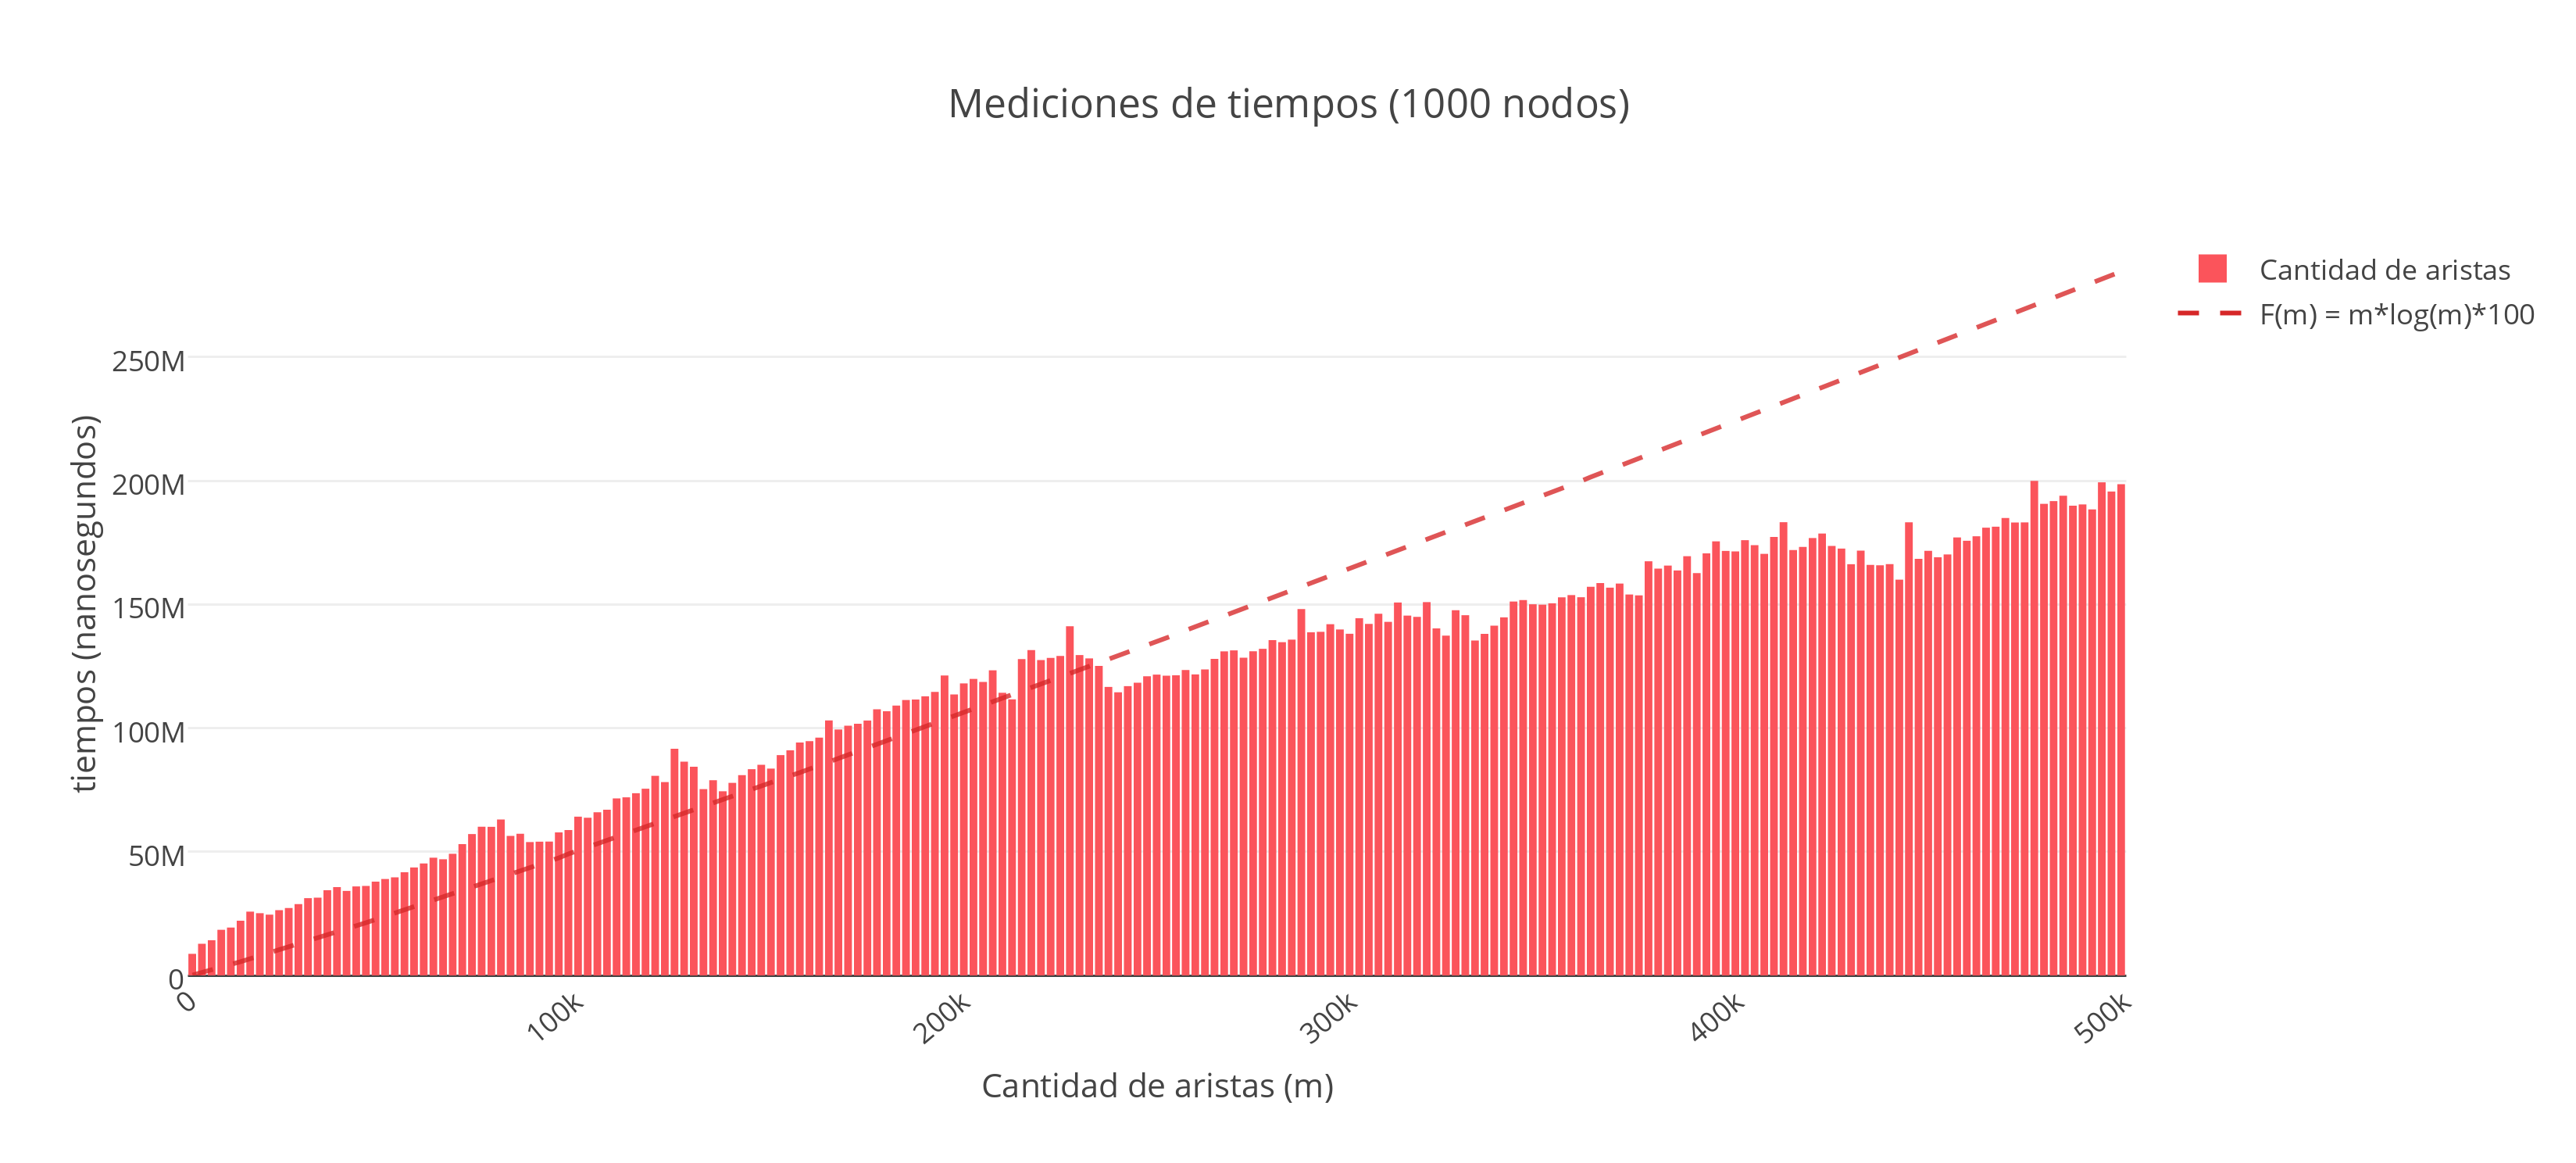
\includegraphics[scale=0.6]{imagenes/ej3/tiempos1000B.png}
% 	\caption{Medición de tiempo promedio con $n$ fijo en 1000}
% 	%\label{tiemposprom}
%  \end{figure}
\newpage
\newpage
\section{Problema 2: Algoritmo Exacto para List Coloring}

\subsection{Descripción de la problemática}
En esta oportunidad se nos pide resolver el problema List Coloring que consiste en (si es posible) colorear un grafo de forma que ningún nodo tenga el mismo color que un nodo adyacente, respetando la lista de colores de cada nodo, lo cual quiere decir que no se le puede asignar un color a un nodo si este no pertenecía a su lista de colores posibles. 

\subsection{Resolución propuesta y justificación}

Para desarrollar un algoritmo exacto para este problema decidimos usar backtracking y de esta forma recorrer todas las opciones de colores y poder encontrar la solución si esta existe.\\

Como el enunciado pide que al llegar a un caso de 2-List Coloring se utilice el algoritmo del primer punto, decidimos cambiar el enfoque de la resolución para poder adaptarlo a instancias del ejercicio 1. Por lo tanto en lugar de usar el enfoque convencional que sería fijar un color para cada nodo y ver si es solución, optamos por recorrer todos los nodos del grafo fijando dos colores por cada uno y al llegar al último nodo llamar a 2-list Coloring para que chequee si con esa configuración de colores hay solución. Si la respuesta es $"X"$ entonces se selecciona el siguiente color del último nodo y se vuelve a probar. Cuando se acaban los colores del último, se elije el próximo color del ante último y se vuelve a empezar de cero con los colores del siguiente y así hasta que se prueben todos los colores de todos los nodos. De esta forma siempre se llega a un caso base que es resoluble por 2-List Coloring.\\

Para evitar repetir colores se utilizan dos iteradores, el primero (\emph{it}) siempre arranca desde el primer color de la lista y el segundo (\emph{it2}) arranca desde el índice siguiente al de \emph{it}. De esta forma se generan todas las permutaciones de dos colores sin repeticiones ni omisiones.


\subsubsection{Podas}

\begin{itemize}
	\item La primer poda que se realiza es la de ordenar la lista de nodos de forma que queden primero los nodos con menor cantidad de colores ya que de esta forma si se eligen los colores de un nodo $a$ con dos colores primero y luego se pasa a uno $b$ de cinco, se estaría recorriendo el subgrafo que no contiene a $a$ dos veces en lugar de las cinco que se recorrería si estuviera primero el nodo $b$.
	\item Una poda también sería no llamar a 2-List Coloring con un nodo que tenga los colores $\{0, 1\}$ y luego volverlo a llamar con el mismo nodo con los colores $\{1, 0\}$ por ese motivo se recorren las listas de colores de la forma que explicamos antes.
	\item En el caso que el nodo original tenga un solo color, se llama directamente a 2-List Coloring, evitando entrar al while.
	\item Si se llega a una solución, se corta el backtracking y se devuelve esa. De esta forma en el caso promedio y mejor, no se recorrería todo el árbol de soluciones ya que no necesita encontrar todas las posibles.
\end{itemize}

\subsection{Análisis de la complejidad}

Para analizar la complejidad utilizaremos el siguiente pseudocódigo, en el cual se utilizan los términos:
\begin{itemize}
	\item \texttt{grafo}: para referirse al que viene por parámetro.
	\item \texttt{grafo2colores}: para el grafo que se construye para pasarselo al algoritmo del problema 1 y que admite hasta 2 colores por nodo.
	\item \texttt{ListColoring}: es el algoritmo que estamos analizando y representa el llamado recursivo a la misma función. 
	\item \texttt{2ListColoring}: es el algoritmo del problema 1 y se usa para obtener la solución a un grafo con a lo sumo dos colores por nodo.
	\item $count$: es una variable pasada por parámetro que se utiliza para avanzar y retroceder en la lista de nodos.
	\item $c\_original$: es la cantidad máxima de colores que puede tener un nodo y que está dada por la entrada del problema.
\end{itemize}

% El pseudocódigo de nuestro algoritmo sin podas es el siguiente:
\begin{algorithm}
\caption{ListColoring Exacto Sin Podas}
\label{lce}
\begin{algorithmic} 

\STATE $count = $ índice en la lista de nodos del \texttt{grafo} (inicializada en cero, viene por parámetro) \COMMENT{$\mathcal{O}(1)$}

\IF {$count ==$ cantidad de nodos del \texttt{grafo}}
	\STATE Llamar a \texttt{2ListColoring} para resolver \texttt{grafo2colores} \COMMENT{$\mathcal{O}(1)$}
	\STATE Retornar 
\ENDIF

\STATE $nodo = $ Obtener el nodo a procesar del \texttt{grafo} con el índice $count$ \COMMENT{$\mathcal{O}(1)$}
\STATE $it = $ Obtener un iterador de la lista de colores de $nodo$ \COMMENT{$\mathcal{O}(1)$}
\STATE $coloresSeleccionados = $ Obtener la lista de colores del $nodo$ en el \texttt{grafo2colores} \COMMENT{$\mathcal{O}(1)$}
\STATE Incrementar $count$ \COMMENT{$\mathcal{O}(1)$}
\WHILE[$\mathcal{O}(c\_original)$ en cantidad de ejecuciones.]{Haya próximo en la lista de colores}
	\STATE $color1 = $ Próximo en la lista \COMMENT{$\mathcal{O}(1)$}
	\STATE $it2 = $ Obtener un iterador que apunta al color que le sigue a $color1$ \COMMENT{$\mathcal{O}(1)$}
	\STATE Asignar $color1$ en la primer posición de la lista $coloresSeleccionados$ \COMMENT{$\mathcal{O}(1)$}
	\WHILE[$\mathcal{O}(c\_original)$ cantidad de ejecuciones]{Haya próximo en la lista de colores a partir de $it2$}
		\STATE $color2 = $ Próximo en la lista a partir de $it2$ \COMMENT{$\mathcal{O}(1)$}
		\STATE Asignar $color2$ en la segunda posición de la lista $coloresSeleccionados$ \COMMENT{$\mathcal{O}(1)$}
		\STATE Llamara a \texttt{ListColoring} con el count ya incrementado %\COMMENT{$\mathcal{O}(1)$}
	\ENDWHILE
\ENDWHILE
\STATE Retornar
\end{algorithmic}
\end{algorithm}

% \subsection{Código fuente}

% A continuación se incluyen las partes más relevantes del código.\\
% La clase \emph{Main.java} se encarga de hacer el backtracking para recorrer todos los nodos fijando de a dos colores:
% \lstinputlisting[name=main, numbers=left, frame=lines, firstline=47, lastline=80]{../ej2/src/Main.java}
% La clase \emph{Lector.java} se encarga de leer el input y transformarlo en dos grafos, uno que contiene todos los colores y el otro que tiene un máximo de dos colores para poder pasarselo como parámetro a \emph{2ListColoring}.
% \lstinputlisting[name=lec, numbers=left, frame=lines, firstline=40, lastline=83]{../ej2/src/Lector.java}
% La clase \emph{Nodo_Coloreable_ej2} es muy similar a la clase \emph{Nodo_Coloreable_ej1}, lo único que cambia es que esta acepta una lista de mas de dos colores.

% \newpage 

% \lstinputlisting[name=nc, numbers=left, frame=lines, firstline=12, lastline=16]{../ej2/src/Nodo\string_Coloreable\string_ej2.java}

% \subsection{Experimentación}

% \subsubsection{Constrastación Empírica de la complejidad}
% \subsubsection{Mejor Caso}
% \subsubsection{Peor caso}

% \begin{figure}[H]
% 	\centering
%  	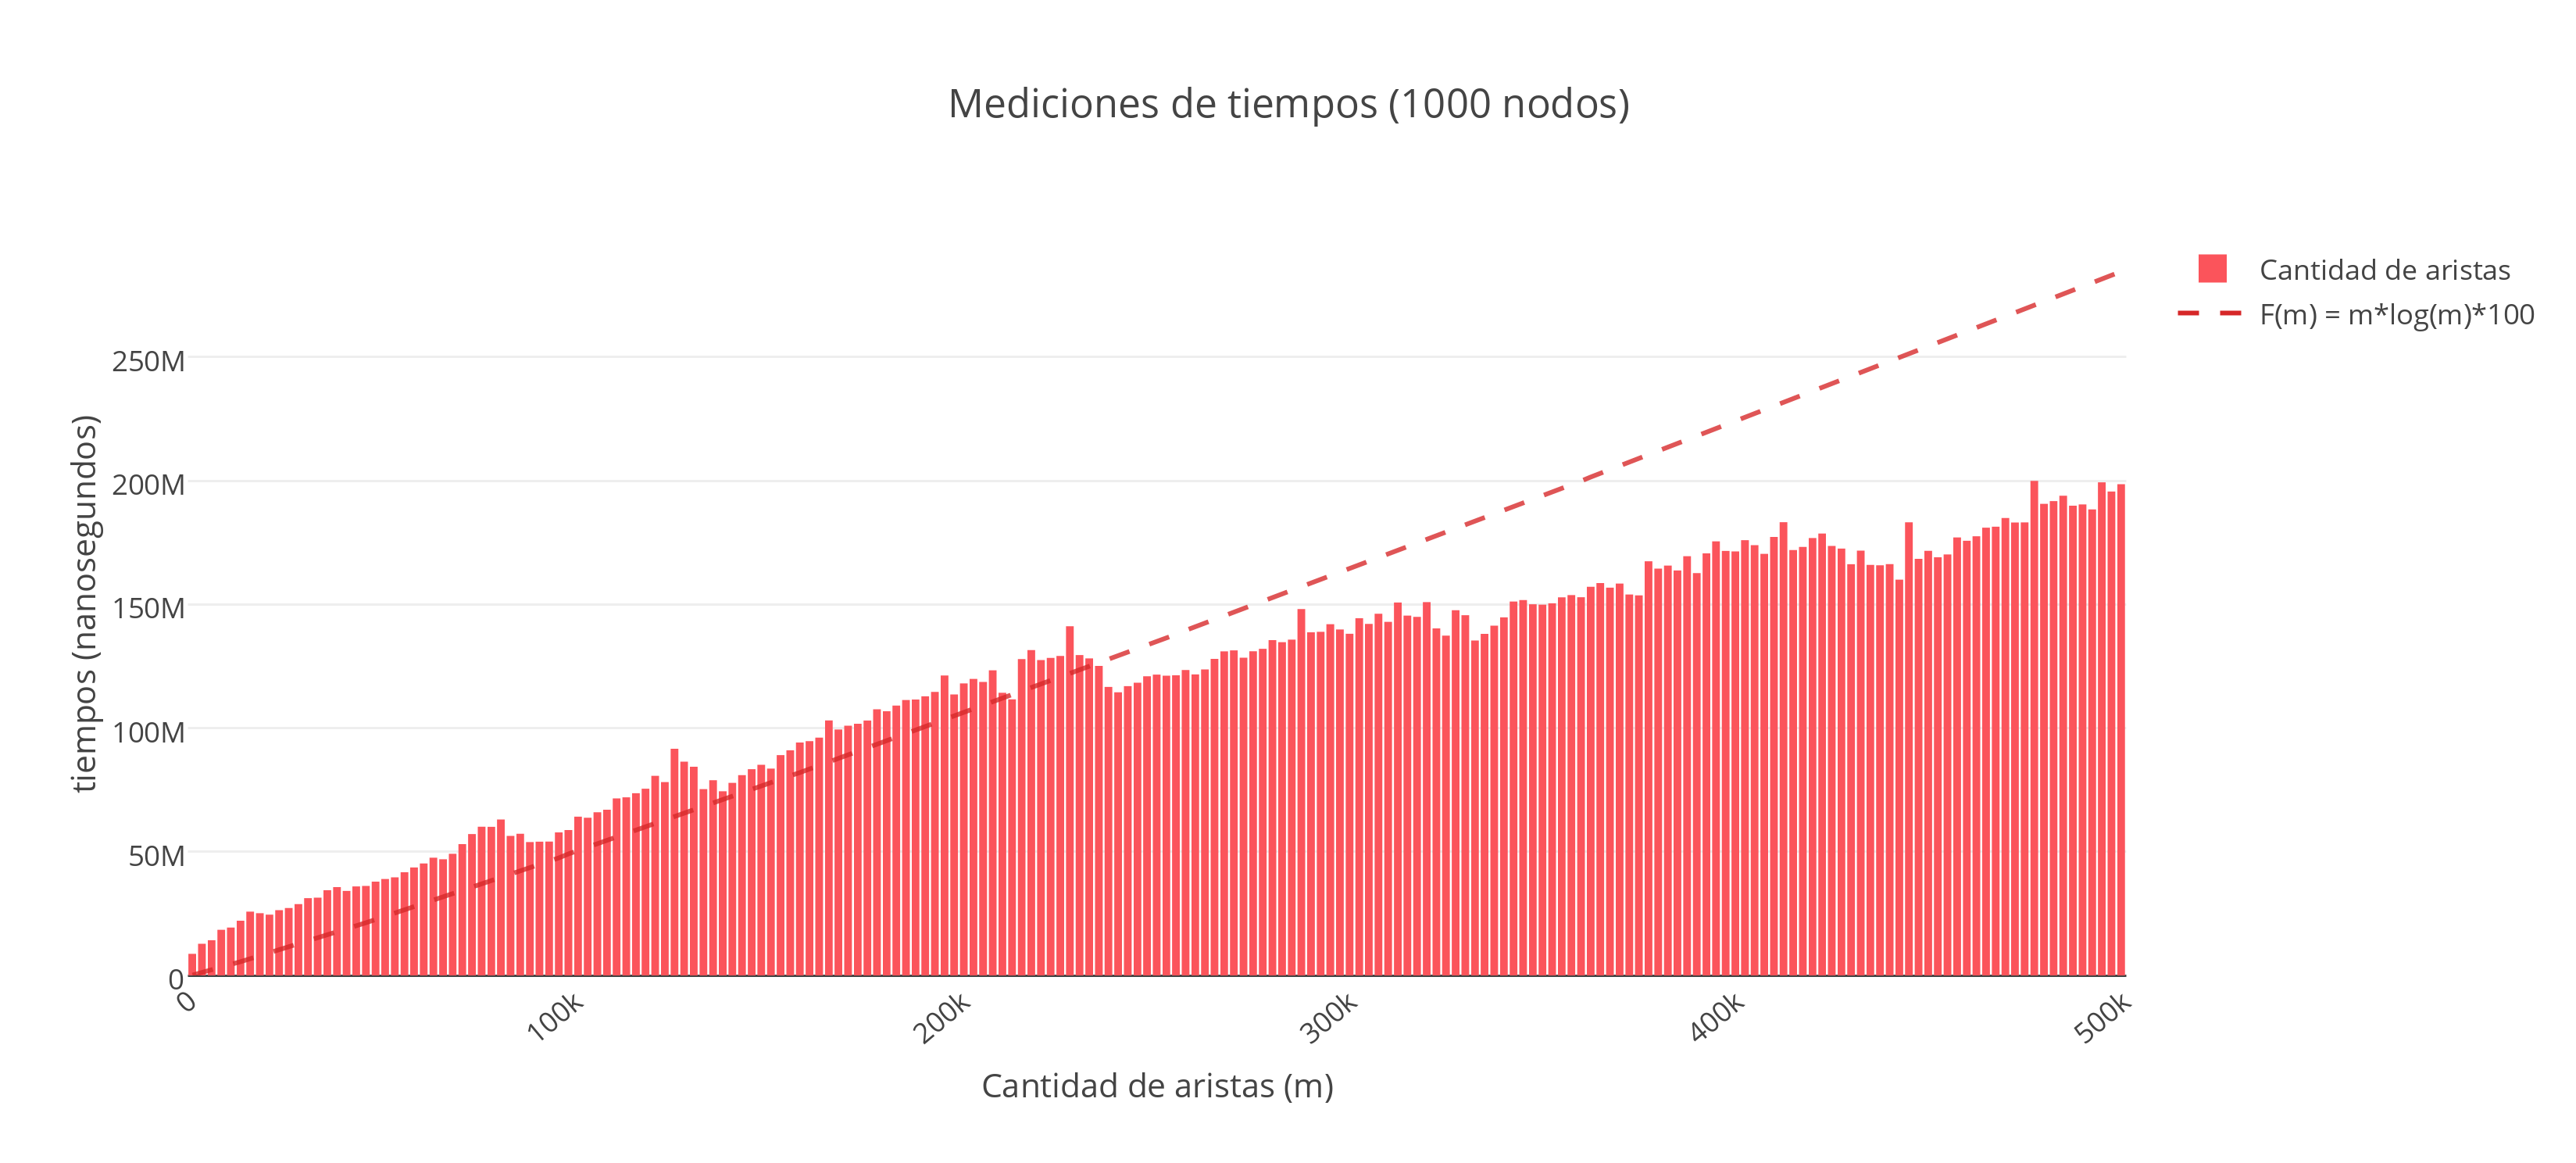
\includegraphics[scale=0.6]{imagenes/ej3/tiempos1000B.png}
% 	\caption{Medición de tiempo promedio con $n$ fijo en 1000}
% 	%\label{tiemposprom}
%  \end{figure}
\newpage
\section{Problema 3: Heurística Constructiva Golosa}

\subsection{Descripción de la problemática}
En esta oportunidad se nos pide colaborar en la asignación de aulas con diversos recursos a un conjunto de materias (con un horario establecido e invariable) que necesitarían hacer uso de ellos durante el dictado de clase.\\
Como en este caso nos interesa distinguir las aulas de acuerdo a sus recursos, le asignaremos a cada una un color y uniremos con aristas aquellas materias que se han querido reservar para horarios cuya intersección no es vacía.\\
Dicho esto, nuestra tarea consiste en generar un algoritmo que implemente una heurística cuyo objetivo sea encontrar alguna forma de colorear los nodos (es decir, asignar a cada materia un aula ), minimizando en la medida de lo posible la cantidad de conflictos (entendidos estos como instancias que impiden que el coloreo generado sea válido, es decir, que verifique para toda arista que a sus nodos adyacentes se les haya asignado distinto color.) 


\subsection{Resolución propuesta y justificación}
Dos ideas de peso sugieron al proponernos resolver este problema:
\begin{itemize}
\item{Iterar sobre el grafo (a lo sumo C-1 veces) descartando de cada uno de los nodos uno de sus colores posibles, escogido mediante una función de peso que decidiera cuál de ellos podría generar más conflictos si se utilizara para colorear al nodo examinado.  }
\item{Realizar un barrido del grafo mediante BFS utilizando una función de peso similar a la mencionada que permitiera decidir para cada nodo cuál sería el color - potencialmente - de menor riesgo en una vecindad reducida y asignárselo. }
\end{itemize}

Un problema emergió al analizar la primera de las ideas: el hecho de que se realizaran varias iteraciones sobre el mismo grafo hacía que al comenzar cada una de ellas cada nodo tuviese más información del grafo completo que la que podía verificar en la anterior. Dicho de otra forma: en la primera iteración cada nodo tomaba la mejor decisión posible en función de su vecindad de primer nivel, pero en las siguientes ya dicha vecindad - ahora modificada de acuerdo a su propio entorno - le proveía al nodo más datos que los alcanzables hasta entonces. Es decir, no cumplía los requisitos para ser catalogado como ``algoritmo goloso''.\\
Es por esto que se decidió implementar la segunda opción, la cuál se explica a continuación:\\
Supóngase que se tiene el siguiente grafo, donde los números dentro de cada nodo indican su índice y los que se encuentran fuera enumeran sus colores posibles.\\

 \begin{figure}[H]
    \begin{center}
  	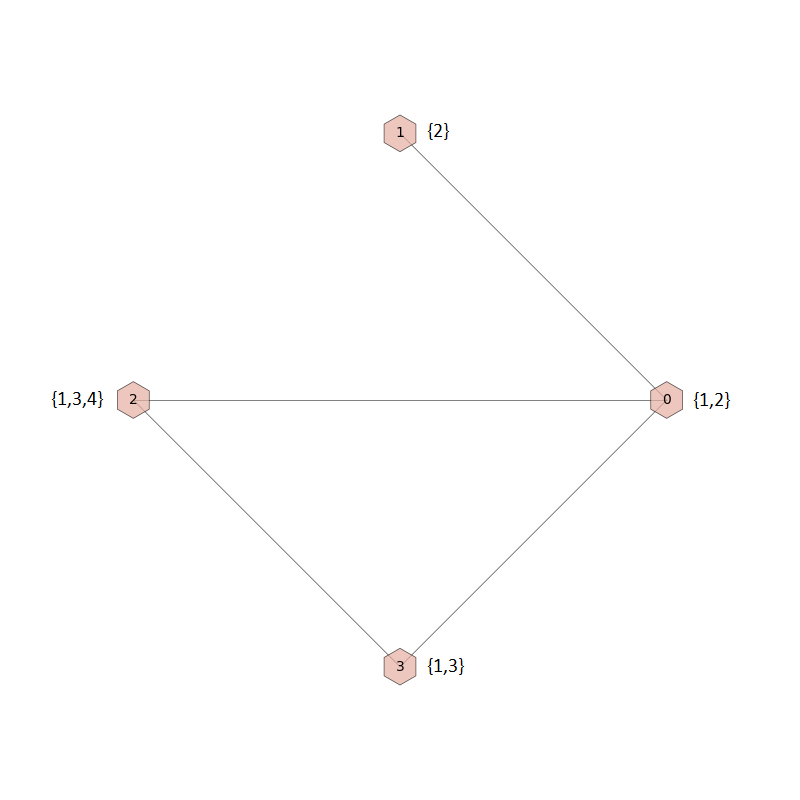
\includegraphics[width=13cm]{imagenes/Ej3/4Nodos0.png}
 	\caption{Grafo sin colorear}
 	\label{sinColor}
    \end{center}
  \end{figure}


Defínase Peso(N$_{c}$) como la función que determina la magnitud del perjuicio ocasionable al elegir colorear el nodo N de color c (con c $\epsilon$ \{colores de N\}), ${X}_{(c,p)}$ como el valor relativo X del color c para el nodo p. Entonces en un primer paso, los valores son los siguientes: 

\begin{itemize}
	\item \textbf{Nodo 0}
	\begin{itemize}
		\item Color 1:
		\begin{itemize}
			\item  $\frac{0}{1}_{(1,1)}$
			\item  $\frac{1}{3}_{(1,2)}$
			\item  $\frac{1}{2}_{(1,3)}$
		\end{itemize}

		\item Color 2:
		\begin{itemize}
			\item  $\frac{1}{1}_{(2,1)}$
			\item  $\frac{0}{3}_{(2,2)}$
			\item  $\frac{0}{2}_{(2,3)}$
		\end{itemize}
	\end{itemize}
\end{itemize}

Por lo tanto, \\
Peso(0$_{1}$) =  $\frac{ \frac{1}{2}_{(1,3)}}{\textbf{2}}$ + $\frac{\frac{1}{3}_{(1,2)}}{\textbf{3}}$ + $\frac{\frac{0}{1}_{(1,1)}}{\textbf{4}}$ $\simeq$ 0.36 \\
Peso(0$_{2}$) =  $\frac{\frac{1}{1}_{(2,1)}}{\textbf{2}}$ + $\frac{\frac{0}{3}_{(2,2)}}{\textbf{3}}$ + $\frac{\frac{0}{2}_{(2,3)}}{\textbf{4}}$ $\simeq$  0.5 \\
\newline
Como Peso(0$_{1}$) $\leq$  Peso(0$_{2}$), el color del que se pintará al nodo es del 1 (tal como se muestra en la \newline 
figura \ref{1color} )

 \begin{figure}[H]
    \begin{center}
  	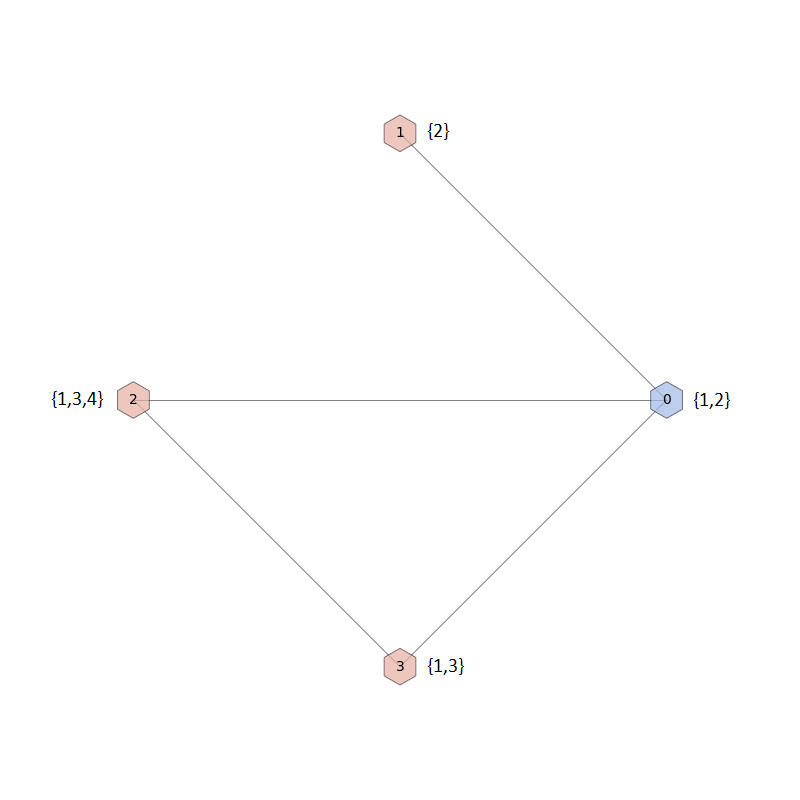
\includegraphics[width=13cm]{imagenes/Ej3/4Nodos1.png}
 	\caption{Al nodo 0 se le asigna el color 1}
 	\label{1color}
    \end{center}
  \end{figure}

Prosigamos con el nodo 1. Su valor es el siguiente:

\begin{itemize}
	\item \textbf{Nodo 1}
	\begin{itemize}
		\item Color 2:
		\begin{itemize}
			\item  $\frac{0}{2}_{(2,0)}$ 
		\end{itemize}
	\end{itemize}
\end{itemize}

Nótese que el valor $\frac{0}{2}_{(2,0)}$ no es $\frac{1}{2}_{(2,0)}$ porque el nodo 0 ya fue coloreado y de un color distinto al 2. Es por esto que al nodo 0 ``no le importa'' que su vecino, el nodo 1, se coloree del color 2 y por lo tanto el peso que retorna para dicho color es \textit{0}. Además, este es el único peso que tiene en cuenta el nodo 1, puesto que no tiene más nodos adyacentes ni otros colores disponibles. Por lo tanto, como se muestra en la figura \ref{2colores}, el nodo 1 se pinta del color 2.

 \begin{figure}[H]
    \begin{center}
  	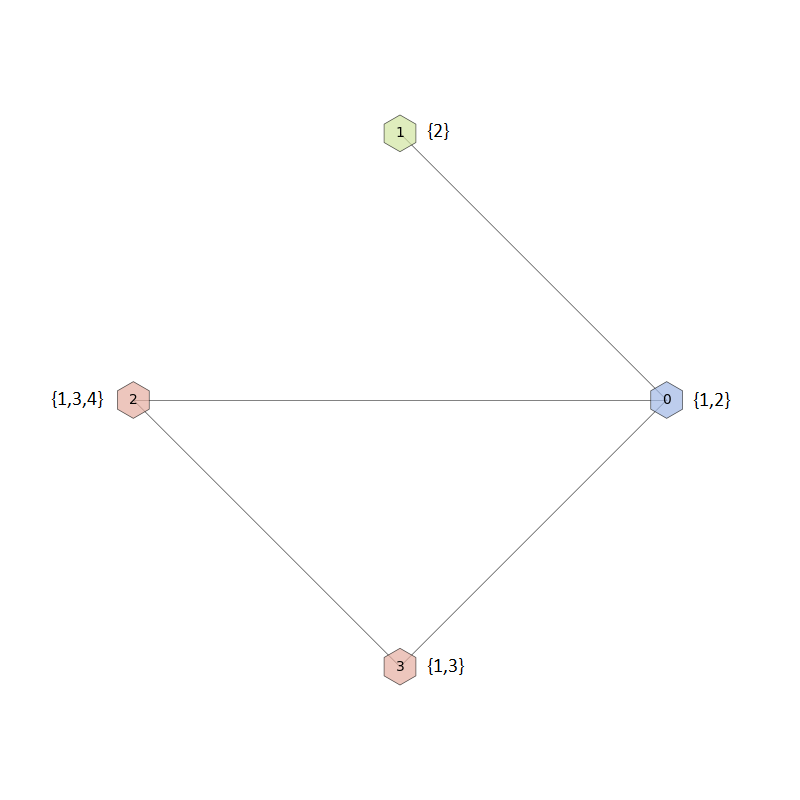
\includegraphics[width=13cm]{imagenes/Ej3/4Nodos2.png}
 	\caption{Al nodo 1 se le asigna el color 2}
 	\label{2colores}
    \end{center}
  \end{figure}

Continuemos el coloreo con el nodo 2: \\

\begin{itemize}
	\item \textbf{Nodo 2}
	\begin{itemize}
		\item Color 1:
		\begin{itemize}
			\item  $\frac{0}{2}_{(1,0)}$
			\item  $\frac{1}{2}_{(1,3)}$
		\end{itemize}

		\item Color 3:
		\begin{itemize}
			\item  $\frac{0}{2}_{(3,0)}$
			\item  $\frac{1}{2}_{(3,3)}$
		\end{itemize}

		\item Color 4:
		\begin{itemize}
			\item  $\frac{0}{2}_{(4,0)}$
			\item  $\frac{0}{2}_{(4,3)}$
		\end{itemize}
	\end{itemize}
\end{itemize}

Nuevamente, los colores posibles del nodo 0 no tienen injerencia a menos que el valor por el que se pregunte sea equivalente al color con el cual se pretende colorear un nodo adyacente.\\
Como en este caso  Peso(2$_{4}$) $\leq$  Peso(2$_{3}$)  $\leq$  Peso(2$_{1}$), se le asigna al nodo 2 el color 4 (ver \ref{3colores})

 \begin{figure}[H]
    \begin{center}
  	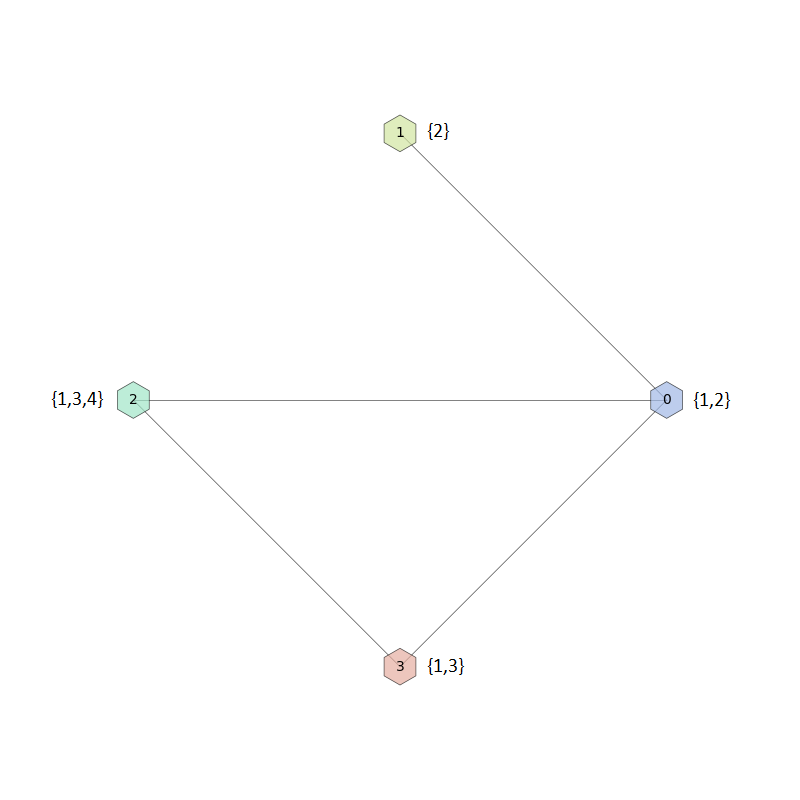
\includegraphics[width=13cm]{imagenes/Ej3/4Nodos3.png}
 	\caption{Al nodo 2 se le asigna el color 4}
 	\label{3colores}
    \end{center}
  \end{figure}

Por último, definamos el coloreo del nodo 3:\\

\begin{itemize}
	\item \textbf{Nodo 3}
	\begin{itemize}
		\item Color 1:
		\begin{itemize}
			\item  $\frac{1}{1}_{(1,0)}$
			\item  $\frac{0}{3}_{(1,2)}$
		\end{itemize}

		\item Color 3:
		\begin{itemize}
			\item  $\frac{0}{2}_{(3,0)}$
			\item  $\frac{0}{3}_{(3,2)}$
		\end{itemize}
	\end{itemize}
\end{itemize}

Obsérvese que $\frac{1}{1}_{(1,0)}$ es distinto del esperado $\frac{1}{2}_{(1,0)}$. Esto se debe a que ell valor escogido representa una medida de la importancia que se le da al nodo ya coloreado ``0''. Como queremos evitar la mayor cantidad de conflictos, ante casos de este estilo se define que el nodo coloreado retorne el valor absoluto ``1'' (recordemos que, cuanto más grande este valor, mayor es la restricción de pintar un nodo de dicho color).\\

De esta forma, queda coloreado todo el grafo como se muestra en la figura \ref{4colores}

 \begin{figure}[H]
    \begin{center}
  	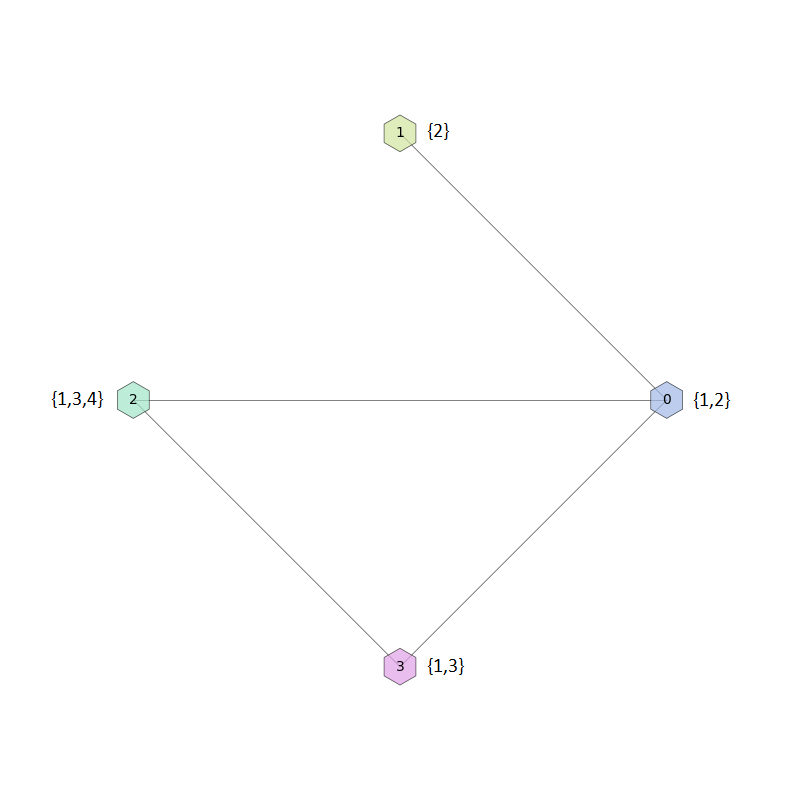
\includegraphics[width=13cm]{imagenes/Ej3/4Nodos4.png}
 	\caption{Al nodo 3 se le asigna el color 3}
 	\label{4colores}
    \end{center}
  \end{figure}


\subsection{Código fuente}

A continuación se incluyen las partes más relevantes del código generado\\

La clase \emph{Lector.java} se encarga de tomar los datos del archivo de entrada y procesarlos para construir el grafo mediante el método \textit{MakeGraph()}:\\

\begin{lstlisting}
	public Grafo MakeGraph() throws IOException 
	{
		Grafo grafo = new Grafo();
		int[] nodosAristasColores = Ej3Utils.ToIntegerArray(this.getArchivo().readLine().split(" "));
		grafo.cantidadDeNodos = nodosAristasColores[0];
		grafo.setCantidadDeAristas(nodosAristasColores[1]);
		grafo.setCantidadDeColores(nodosAristasColores[2]);
		
		try { grafo.setNodos(this.ObtenerListaDeNodos(grafo.cantidadDeNodos, grafo.getCantidadDeColores()));} 
		catch (IOException e) { System.out.println("Se produjo un error al generar los nodos del grafo.");}
		boolean[][] matrizDeAdyacencia = GenerarMatrizDeAdyacencia(grafo.getCantidadDeNodos(), grafo.getCantidadDeAristas(), false);
		grafo.setListaDeAdyacencia(Ej3Utils.matrizDeAdyacenciaToListDeAdyacencia(matrizDeAdyacencia, grafo.getNodos()));
		
		return grafo;
	}
		
\end{lstlisting}


La clase \emph{Grafo.java} contiene el método \textit{MakeRainbow()} que colorea el grafo con la heurística \newline propuesta: \\

\begin{lstlisting}
	public void MakeRainbow() // O(n^2*c*log(n))
	{
		int nodosPintados = 0;
		LinkedList<Nodo> colaNodos = new LinkedList<Nodo>();

		while(nodosPintados < this.cantidadDeNodos)
		{
			colaNodos.add(PicANode(this)); //O(1)
			
			while (!colaNodos.isEmpty()) //O(n)
			{
				Nodo nodoActual = colaNodos.removeFirst(); //O(1)
				
				if (!nodoActual.isVisitado())
				{
					colaNodos.addAll(this.getVecinosDe(nodoActual)); //O(n)
					LinkedList<Integer> coloresRestantes = nodoActual.getColoresRestantes(); //O(1)
					PintarNodo(nodoActual, coloresRestantes, this); //O(c*n*log(n))
					nodosPintados ++;
					nodoActual.setVisitado(true); //O(1)
				}
			}
		}
	}
	
	private static Nodo PicANode(Grafo grafo) 
	{
		Nodo next = new Nodo();
		for(Nodo nodo : grafo.getNodos())
		{
			if (!nodo.isVisitado())
			{
				next = nodo;
				break;
			}
		}
		return next;
	}
	
	private static void PintarNodo(Nodo nodoActual, LinkedList<Integer> coloresRestantes, Grafo grafo) //O(c*n*log(n))
	{
		int colorAPintar = CalcularColorMenosPerjudicial(nodoActual, grafo); //O(c*n*log(n))
		nodoActual.setColor(colorAPintar); 
	}

	private static int CalcularColorMenosPerjudicial(Nodo nodoActual, Grafo grafo) //O(c*n*log(n))
	{
		Double pesoColor = 1.0;
		int colorAPintar = -1;
		for (int color : nodoActual.getColoresRestantes()) //O(c)
		{
			Double peso = CalcularPeso(color, grafo.getVecinosDe(nodoActual)); //O(nlog(n))
			if (peso <= pesoColor)
			{
				pesoColor = peso;
				colorAPintar = color;
			}	
		}	
		return colorAPintar;
	}


	private static Double CalcularPeso(int color, List<Nodo> vecinos) 
	{
		ArrayList<Double> pesos = new ArrayList<Double>();
		for (Nodo nodo : vecinos) //O(n)
		{
			if (nodo.LeImportaQueSuVecinoSePinteDelColor(color)) //O(1)
					pesos.add(nodo.PeligroDePintarUnVecinoDelColor(color));//O(1)(amortizado)
					
		}
		Collections.sort(pesos); //O(nlog(n))
		Double pesoTotal = 0.0;
		for (int k = 0; k < pesos.size(); k++) //O(n)
			pesoTotal += pesos.get(k)/(k+2); //O(1)
		
		return pesoTotal;
	}
		
\end{lstlisting}


\subsection{PseudoCódigo y Análisis de la complejidad}

A continuación se presenta el pseudocódigo del coloreo implementado:

\begin{algorithmic} 
\WHILE{nodos pintados $\leq$ cantidad de nodos //O(n)} 
	\STATE {Elegir un nodo no visitado del grafo // O(n)}
	\STATE {Encolarlo //O(1)}
	\WHILE{hay elementos en la cola}  
		\STATE {Tomar el primer elemento de la cola //O(1)}
		\IF {no fue coloreado //O(1) } 
			\STATE{ Agregar a todos sus vecinos a la cola //O(n)}
			\STATE {Pintar nodo //O(n*c*log(n))}
		\ENDIF
	\ENDWHILE
\ENDWHILE
\end{algorithmic}


El ciclo principal (el externo) tiene razón de ser porque dentro del bucle anidado sólo se colorea una componente conexa por el grafo que recibimos puede ser no conexo, por lo tanto debemos iterar sobre las distintas componentes. Verificando que el algoritmo funcione hasta que la cantidad de nodos pintados sea efectivamente la cantidad de nodos total, y escogiendo cada vez un nodo de una componente no visitada podemos asegurarnos de que el coloreo se realiza sobre la totalidad del grafo.\\
El método \textit{PintarNodo()} tiene como cota superior O(n*c*log(n)). Como se puede ver en el código, dicha complejidad la alcanza al calcular el color menos perjudicial (método \textit{CalcularColorMenosPerjudicial(nodo V,grafo G)}). Mediante el mismo, se calcula el peso de cada color posible C de V mediante la verificación de la existencia de C entre el conjunto de los colores posibles de cada uno de sus nodos adyacentes a V. Gracias a que cada nodo lleva un array de booleanos que responde a dicha operación en O(1), la cota no es mayor.\\
Como la condición de que el nodo no haya sido visitado se valida exactamente n veces y cada vez se agregan a lo sumo n-1 elementos a la cola (con un costo O(1) cada uno), dicha parte del algoritmo cuesta O(n$^{2}$). Sin embargo un costo mayor se paga al ejecutar el método \textit{PintarNodo()}: n veces O(n*c*log(n)) . Esto hace que la complejidad final del algoritmo ascienda a O(n$^{2}$*c*log(n)).

\subsection{Experimentación}
Nos interesa analizar cómo se comporta nuestro algoritmo en función de ciertas características del grafo a ser coloreado: su cantidad de nodos, su cantidad de aristas y el número máximo de colores que puede llegar a tener como opción cada uno de sus nodos.\\
 Es por ello que nuestro primer experimento consistió en evaluar el tiempo necesario para el cómputo de distintos grafos en los cuales se incrementó paulatinamente la cantidad de nodos. Los resultados se pueden observar en la figura \ref{nodostiempo}

 \begin{figure}[H]
    \begin{center}
  	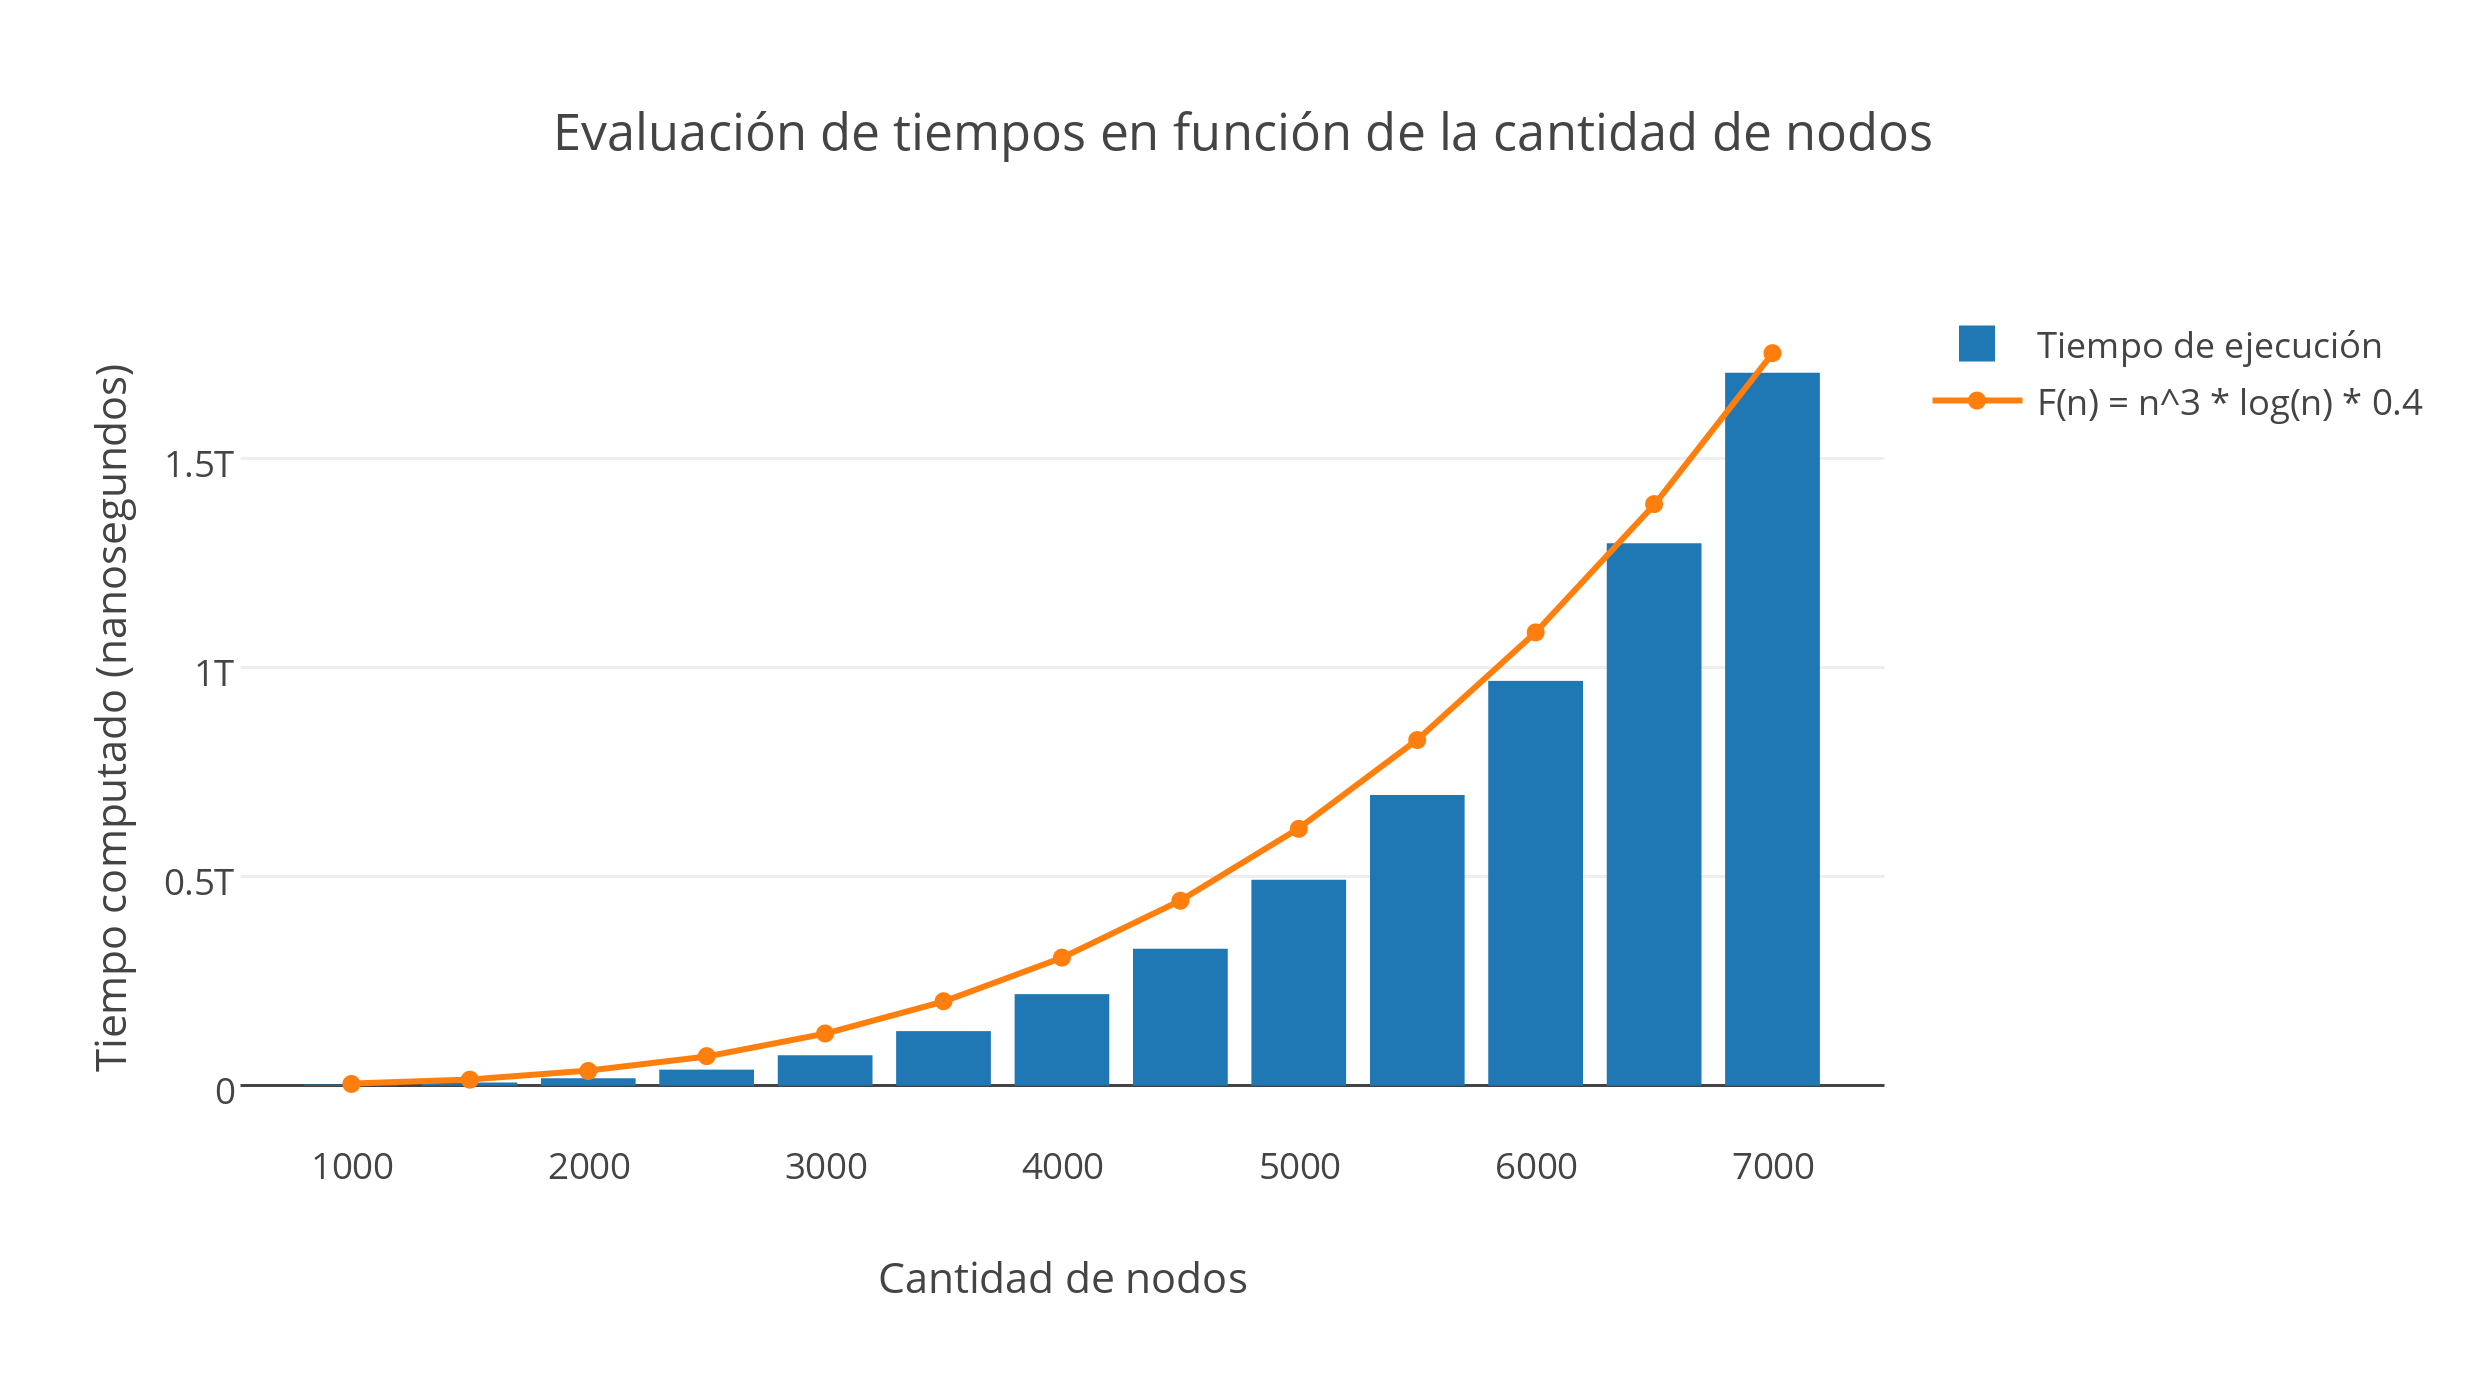
\includegraphics[width=18cm]{imagenes/Ej3/nodostiempo.png}
 	\caption{Tiempos de cómputo en función de la cantidad de nodos}
 	\label{nodostiempo}
    \end{center}
  \end{figure}

Como se puede observar, la función que permite acotar los resultados obtenidos se aproxima asintóticamente a los calculados previamente en forma teórica para estas instancias.\\
Por otro lado, generamos grafos que diferían entre sí únicamente en su cantidad de aristas. Al medir los tiempos obtuvimos los resultados que se exponen en la figura \ref{aristastiempo}

 \begin{figure}[H]
    \begin{center}
  	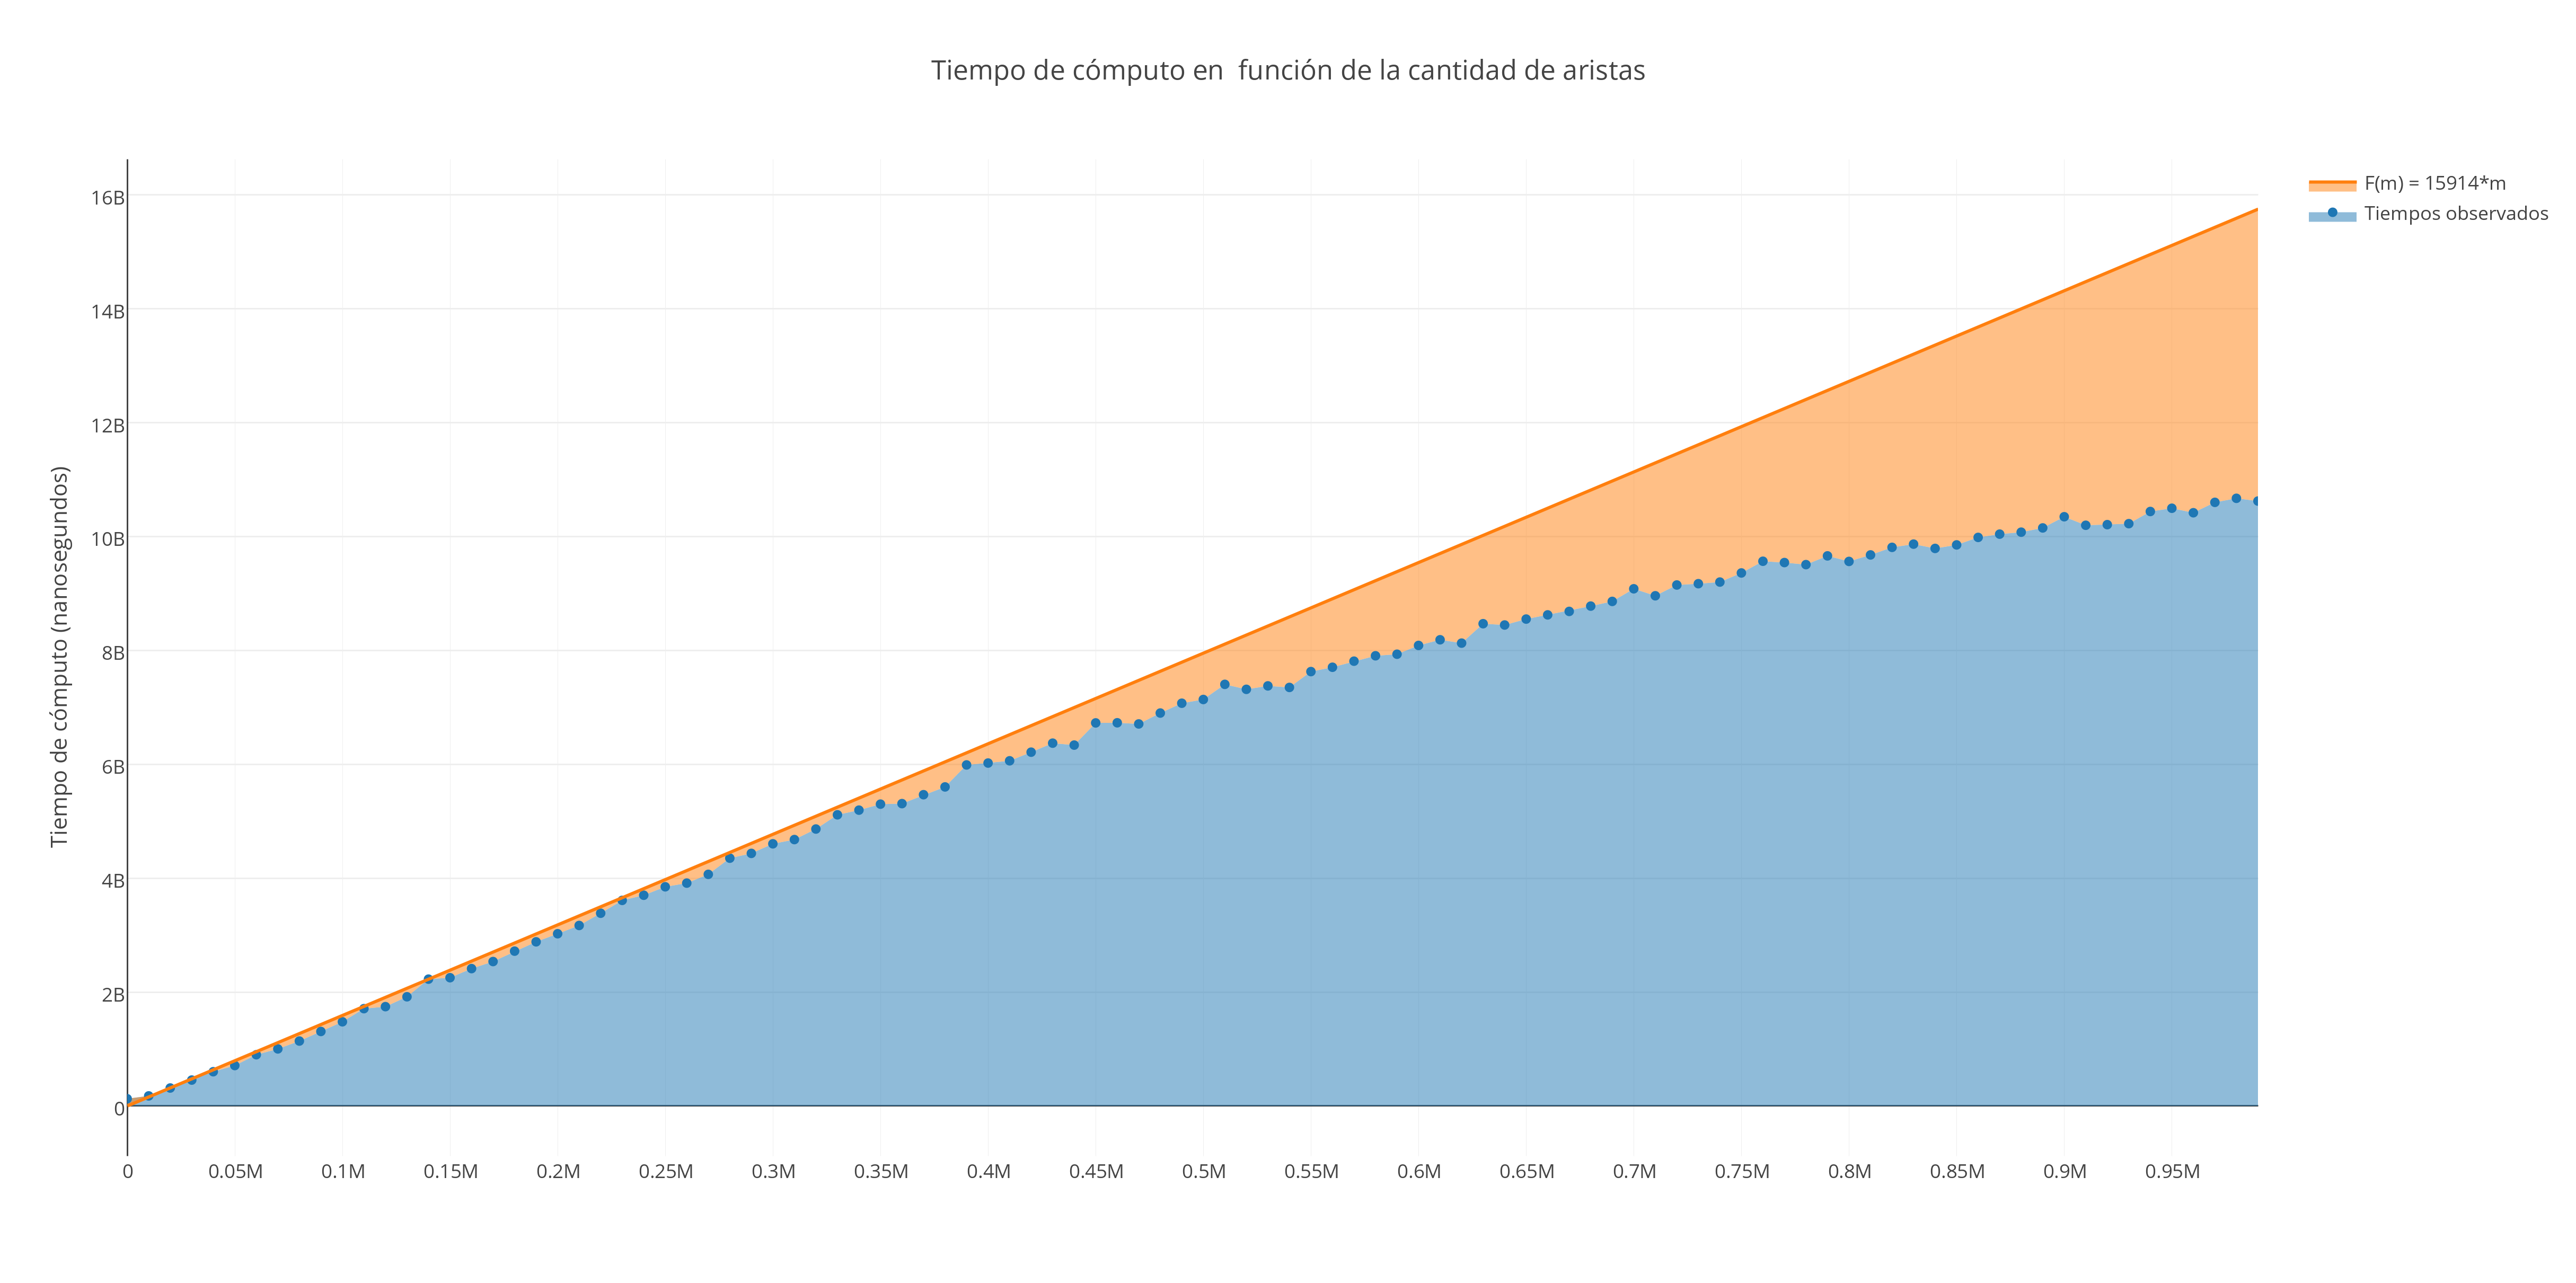
\includegraphics[width=18cm]{imagenes/Ej3/aristastiempo.png}
 	\caption{Tiempos de cómputo en función de la cantidad de aristas}
 	\label{aristastiempo}
    \end{center}
  \end{figure}

Así mismo, realizamos una serie de experimentos en los que modificamos para cada grafo la cantidad máxima de colores que cada uno de ellos podía tener. Con los resultados obtenidos se generó la ilustración \ref{colorestiempo}

 \begin{figure}[H]
    \begin{center}
  	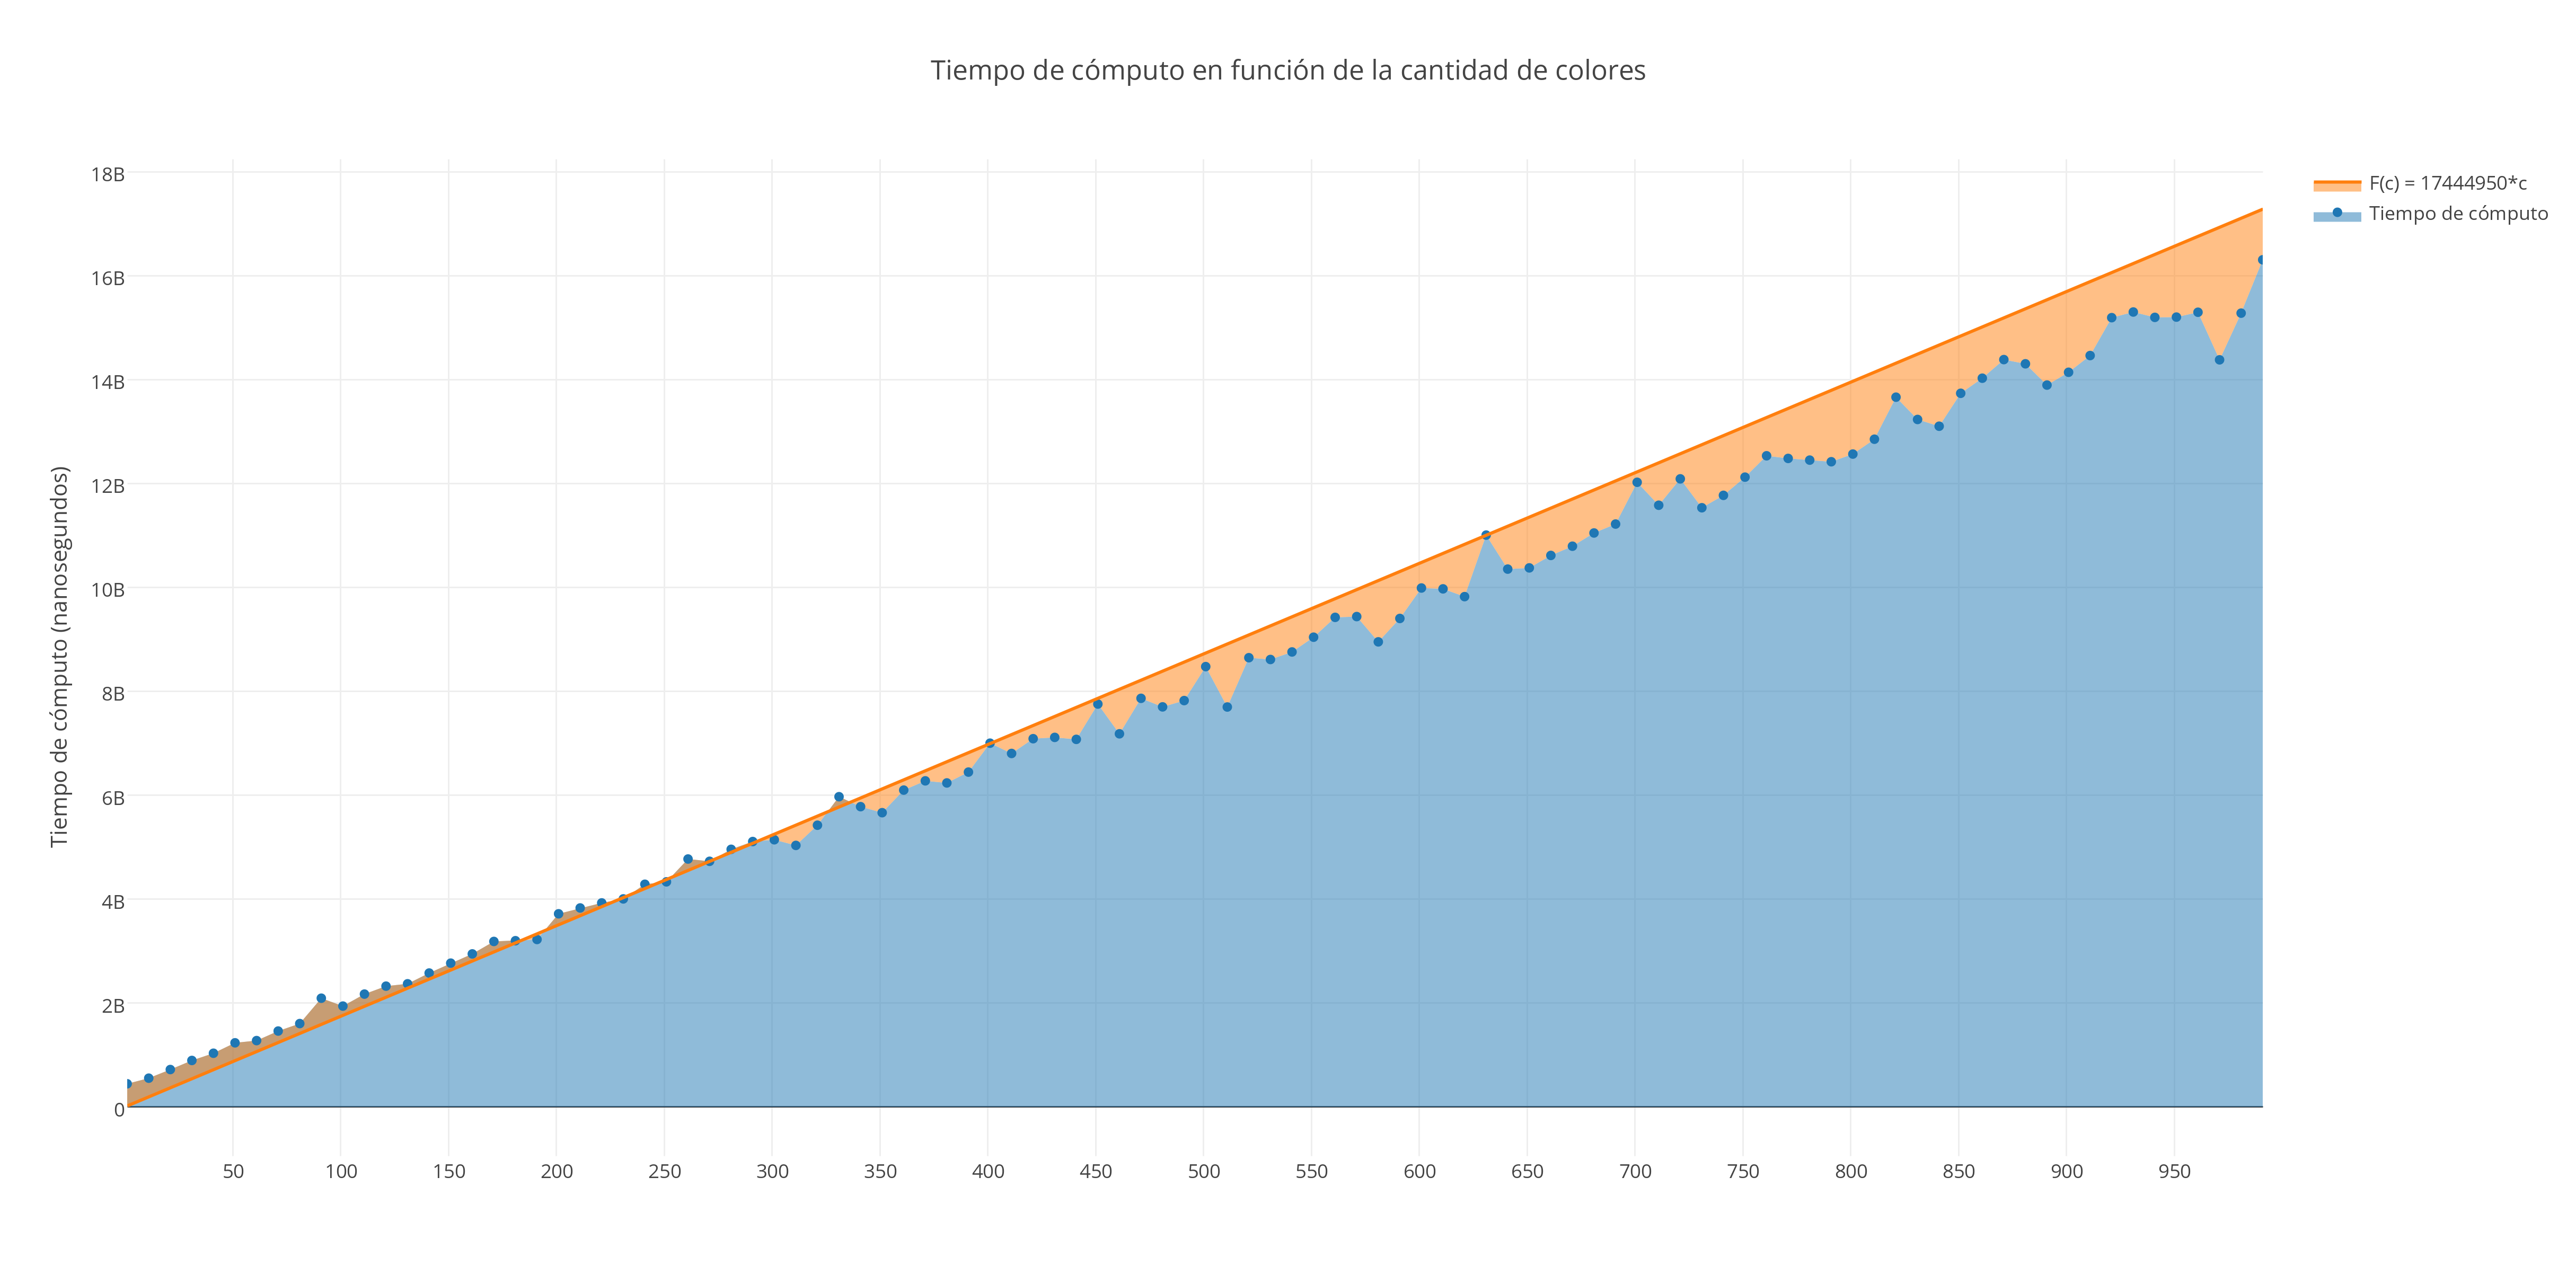
\includegraphics[width=18cm]{imagenes/Ej3/colorestiempo.png}
 	\caption{Tiempos de cómputo en función de la cantidad de colores}
 	\label{colorestiempo}
    \end{center}
  \end{figure}

La misma parece indicar que el tiempo de cómputo dependiera linealmente de la cantidad de colores máxima del grafo. Para entenderlo, hay que considerar que la elección de un color para cada vértice implica haber recorrido cada uno de sus colores. Es decir, es necesario hacer N veces C (a lo sumo). De esta forma, al incrementar la cantidad de colores se realiza una iteración más costosa por cada nodo que no deja de ser lineal.\\

Por último analizamos qué ocurre con la cantidad de conflictos presentes luego del coloreo en función de la cantidad de colores disponibles para realizarlo. Tal como esperábamos a medida que se incrementa el módulo del conjunto de colores, disminuye la cantidad de conflictos. \\
En este caso los resultados resultan intuitivos, puesto que si se dispone de un único color entonces todos aquellos nodos que tengan adyacentes generarán conflictos, puesto que todos ellos tienen una única opción para colorearse. En contrapartida, sabemos que cualquier grafo requiere para ser coloreado a lo sumo tantos colores como cantidad de vértices contenga. En un punto intermedio, como cada nodo tiene potencialmente una cantidad de restricciones intermedia, también la cantidad de conflictos se espera que sea media (es decir, si dos nodos adyacentes comparten colores, siempre existe la posibilidad de que elijan uno distinto cada uno)  \\
Los resultados se pueden observar en la imagen \ref{coloresconflicto}


 \begin{figure}[H]
    \begin{center}
  	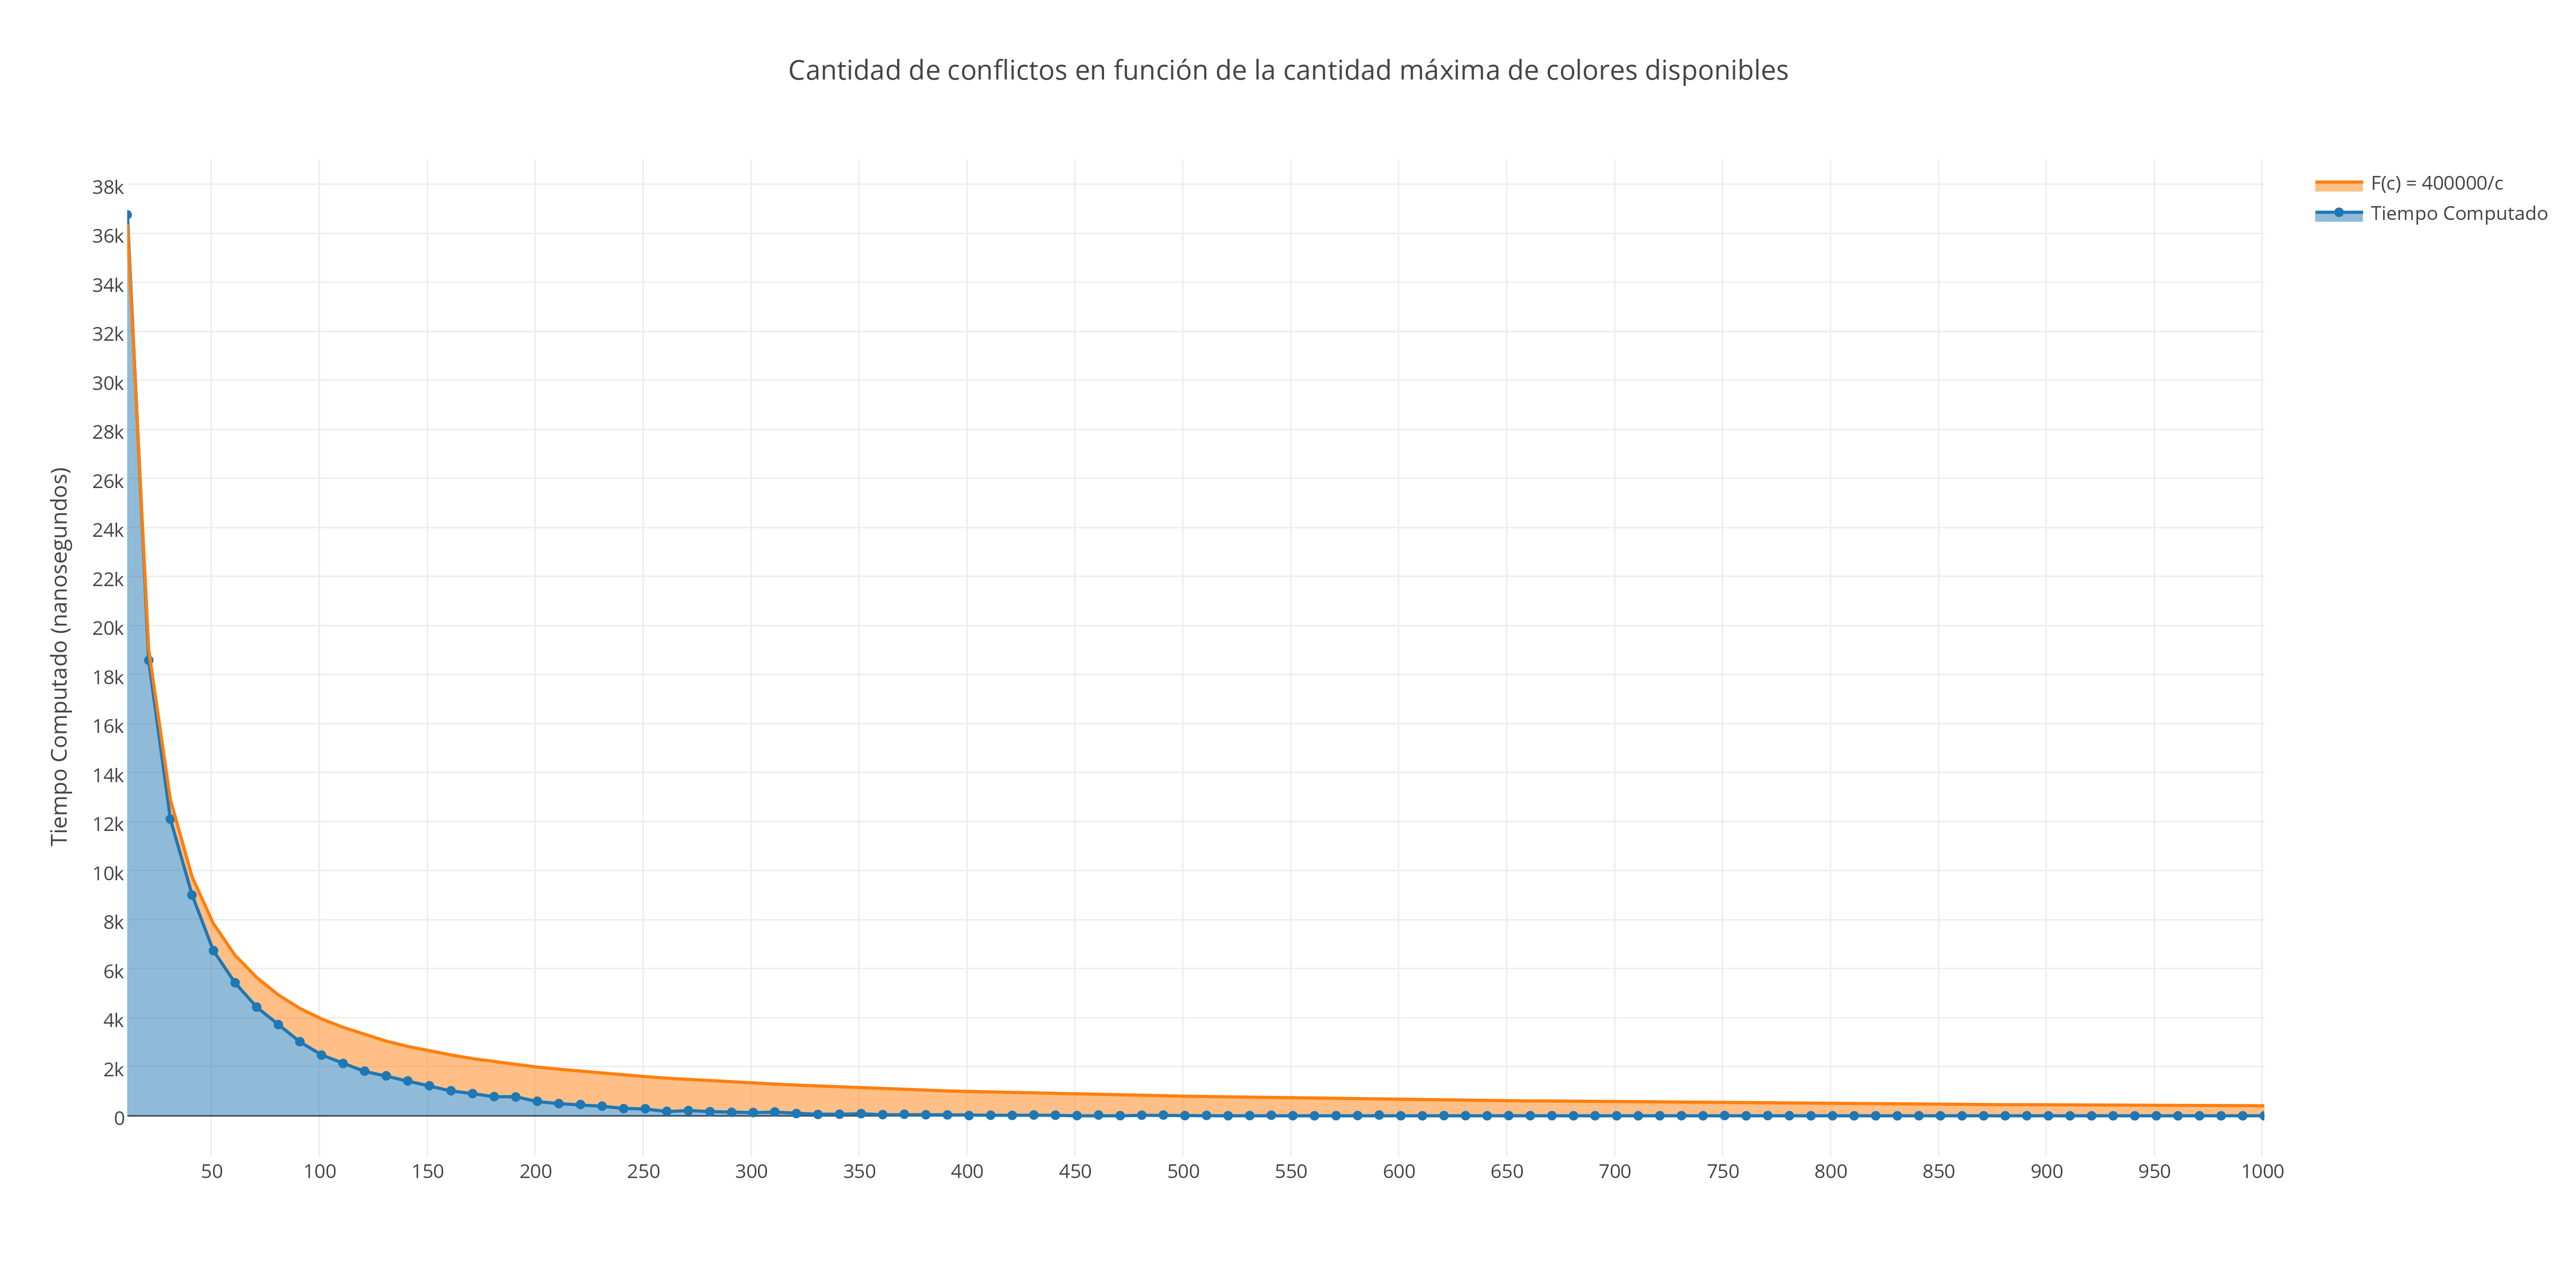
\includegraphics[width=18cm]{imagenes/Ej3/coloresconflicto.png}
 	\caption{Total de conflictos en función de la cantidad de colores máxima}
 	\label{coloresconflicto}
    \end{center}
  \end{figure}

\subsubsection{Peor caso}
Considerando la heurística propuesta, el peor caso a considerar es aquel en que todos los nodos tienen n - 1 nodos adyacentes (es decir un grafo completo). En esta situación el método PintarNodo() - que  se encarga de decidir qué color de los disponibles parecería el apropiado para cada vértice - cumple la cota teórica propuesta, pues debe hacer tantas operaciones como cantidad de vecinos del nodo que  se examina.\\

Además se debe considerar la relación entre la cantidad de colores y la de nodos, puesto que al estar la complejidad fuertemente influida por ambos valores, el que determine finalmente los tiempos de ejecución en el peor caso será aquel cuya cota inferior sea la mayor entre ambas. En otras palabras, si el valor de C fuese equivalente en cada caso a $N^{N}$  (un caso irrisorio - dado que cualquier grafo necesita a lo sumo N colores para colorearse - pero posible) entonces la cota superior estaría determinada en última instancia por el valor de C, absorbiendo asintóticamente la complejidad aportada por N. \\
Por el contrario, si C fuese menor que la cantidad de vértices entonces la cota superior de la heurística propuesta pertenecería a O( $N^{3}$ * log (N) )


\subsubsection{Mejor caso}
Por lo antedicho, el mejor caso se constituye tomando un grafo donde todos sus vértices son aislados. De esta manera, todos y cada uno de ellos podría ser coloreado indistintamente con cualquiera de sus colores disponibles. Sin embargo el conjunto de colores seguiría siendo iterado en su totalidad.



\newpage

% !TEX root = ./informe.tex
\section{Problema 4: Heurística de búsqueda local}

\subsection{Descripción del algoritmo}

Después de aplicar la heurística de búsqueda golosa sobre el problema obtenemos un grafo en el que puede haber conflictos. Esta segunda heurística que desarrollamos se aplica sobre instancias del problema donde ya hay un color válido asignado a todos los nodos. Se trata, entonces, de reducir la cantidad de conflictos de la instancia.

La heurística de búsqueda local define una "vecindad" del problema como una modificación pequeña que se hace sobre el grafo, haciendo un análisis local sobre un nodo o arista. Hemos definido dos vecindades del problema.

El cuerpo principal del algoritmo itera por todos los conflictos del grafo, aplicando una vecindad sobre cada arista que representa a un conflicto.

\subsubsection{Vecindad 1}

Esta vecindad toma una arista en conflicto\footnote{Es decir que ambos nodos de la arista tienen el mismo color.} e intenta modificar el color de uno de los dos nodos, tratando de reducir la cantidad total de conflictos.

\begin{algorithm}[H]
\caption{Vecindad 1.}
\label{vecindad1 pseudocode}
La vecindad opera sobre una arista que recibe como parámetro. Llamaremos a esta arista \texttt{conflicto}. Los dos nodos unidos por esta arista serán N1 y N2:
\begin{enumerate}
 \item crear un diccionario para ambos nodos. El diccionario tendrá como key a los colores del nodo, y como valor una lista de vecinos del nodo que tienen asignado ese color. Llamaremos a estos diccionarios \texttt{conflictosPorColorN1} y \texttt{conflictosPorColorN2}.
 \item tanto para N1 como para N2, iteramos sobre su lista de colores posibles y llenamos los diccionarios conflictosPorColorN1 y conflictosPorColorN2 de manera tal que para cada color posible de ambos nodos, tenemos una lista vacía de vecinos.  // O(c), pues cada nodo tiene a lo sumo $c$ colores posibles.
 \item Luego iteramos la lista de vecinos de N1. Si el color del vecino es uno de los colores posibles de N1, agregaremos este vecino a la lista de conflictosPorColorN1[color_del_vecino]. // O($n$), pues cada nodo tiene a lo sumo $n-1$ vecinos.
 \item Hacemos lo mismo para los vecinos de N2. // O(n)
 \item Ahora buscamos dentro de conflictosPorColorN1 al color que genera menos conflictos (su lista es la más corta). // O(c)
 \item Hacemos lo mismo para conflictosPorColorN2. // O(c)
 \item De esos dos elegimos al menor. Si la cantidad de conflictos es menor a la que se tiene dejando todo como está, cambiamos el color del nodo. Si no, la vecindad no sirvió y no hacemos modificaciones en el grafo. // O(n), ya que para modificar el color de un nodo debemos actualizar una estructura de datos que tiene 
\end{enumerate}
\end{algorithm}


La complejidad calculada para la vecindad 1 es de $\mathcal{O}(n + c)$.


\subsubsection{Vecindad 2}

Esta vecindad toma una arista en conflicto e intenta intercambiar el color de uno de los nodos del confclito con el color de algún vecino suyo.

\begin{algorithm}[H]
\caption{Vecindad 2.}
\label{vecindad2 pseudocode}
La vecindad opera sobre una arista que recibe como parámetro. Llamaremos a esta arista \texttt{conflicto}. Los dos nodos unidos por esta arista serán N1 y N2:
\begin{enumerate}
 \item Para cada N de \{ N1, N2 \} hacemos:
 \begin{enumerate}
   \item obtengo una lista de vecinos de N con los cuales puedo intercambiar color. Son aquellos vecinos que cumplen las siguientes tres condiciones:	// O(n) iteraciones
   \begin{enumerate}
    \item Su color es distinto del color de N.			// O(1)
    \item Su color está dentro de la lista de colores posibles de N	// O(c)
    \item Tienen al color de N dentro de su lista de colores posibles.	// O(c)
   \end{enumerate}
   \item Para cada vecino de N con el que puedo intercambiar color, calculo la cantidad de conflictos que solucionaría al hacer ese intercambio de colores. // O($n^2$)
   \item Elijo al vecino que me solucionaría la mayor cantidad de conflictos. // O(n)
 \end{enumerate}
 \item De entre los dos intercambios posibles (N1 por su vecino, o N2 por su vecino), elijo el que solucione la mayor cantidad posible de conflictos. // O(1)
 \item Realizo el cambio, actualizando la lista de conflictos del grafo.\footnote{Es posible que no encuentre vecinos que solucionen conflictos, o que hacer el intercambio de colores me genere más conflictos que los que previamente tenía. En ese caso, no se realiza el cambio.} // O(n)
 
\end{enumerate}
\end{algorithm}

La complejidad calculada para la vecindad 2 es de $\mathcal{O}(n \cdot c + n^2)$.

\subsubsection{Cantidad total de iteraciones}

Como dijimos, el cuerpo principal del algoritmo itera sobre todos los conflictos hallados al inicio. Con lo cual, la complejidad total del algoritmo debe ser de $\mathcal{O}(conflictos \cdot (n+c)$ para la vecindad 1, y $\mathcal{O}(conflictos \cdot (n \cdot c + n^2))$ para la vecindad2. Y siempre la cantidad de conflictos es $\mathcal{O}(m)$.

\subsection{Experimentación}

\subsubsection{Tiempos de ejecución}

Para verificar experimentalmente las cotas de complejidad calculadas, escribimos generadores de grafos al azar y ejecuciones donde vamos generando grafos y resolviéndolos, tomando mediciones. Se puede hallar el código utilizado en el archivo \texttt{ExperimentosComplejidad.java}.

En primer lugar hicimos un análisis en función de la cantidad de nodos con grafos completos. Esto se puede observar en las figuras \ref{nodosEj4-v1} y \ref{nodosEj4-v2}. Allí se ve que los tiempos medidos para la vecindad 1 incrementan dentro de la cota definida por la curva de $n^3$. Esto es razonable ya que en un grafo completo la cantidad de aristas es del órden de $n^2$, y la cantidad máxima de colores se dejó fija para estas mediciones.

Los tiempos de la vecindad 2 se ve que incrementan dentro de la cota definida por la curva de $n^4$, lo cual también se condice con la complejidad calculada a partir del código, ya que en un grafo completo $\mathcal{O}(m \cdot (n^2 + n \cdot c)) \in \mathcal{O}(n^2 (n^2 + n \cdot c))$

\begin{figure}[H]
	\centering
 	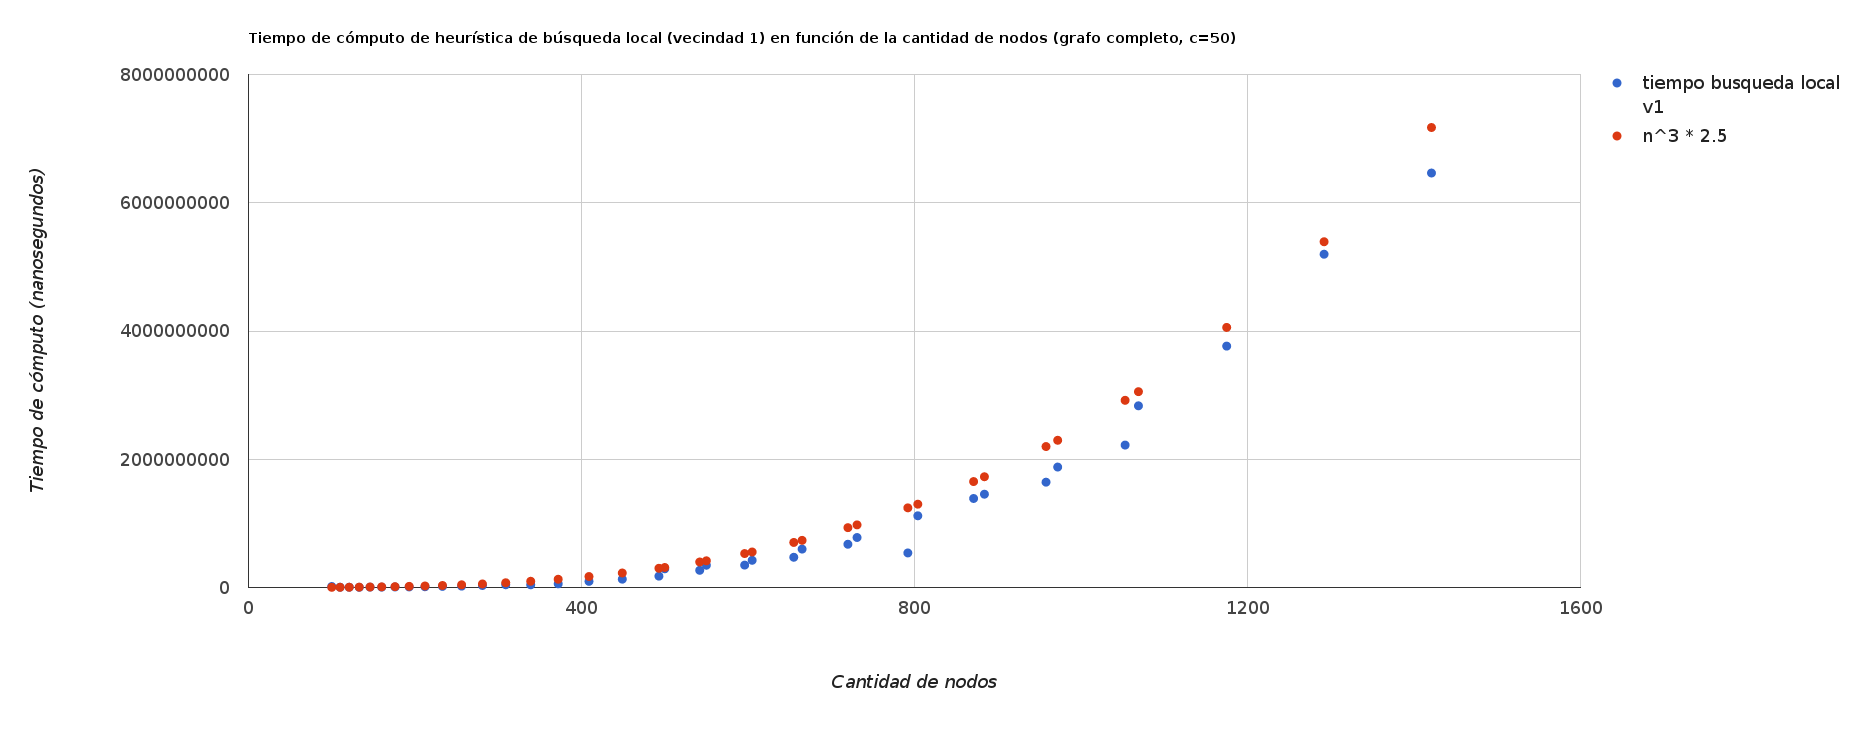
\includegraphics[width=18cm]{imagenes/Ej4/TvsNodosV1.png}
	\caption{Tiempos de cómputo en vecindad 1 en función de la cantidad de nodos.}
	\label{nodosEj4-v1}
 \end{figure}
 
 \begin{figure}[H]
	\centering
 	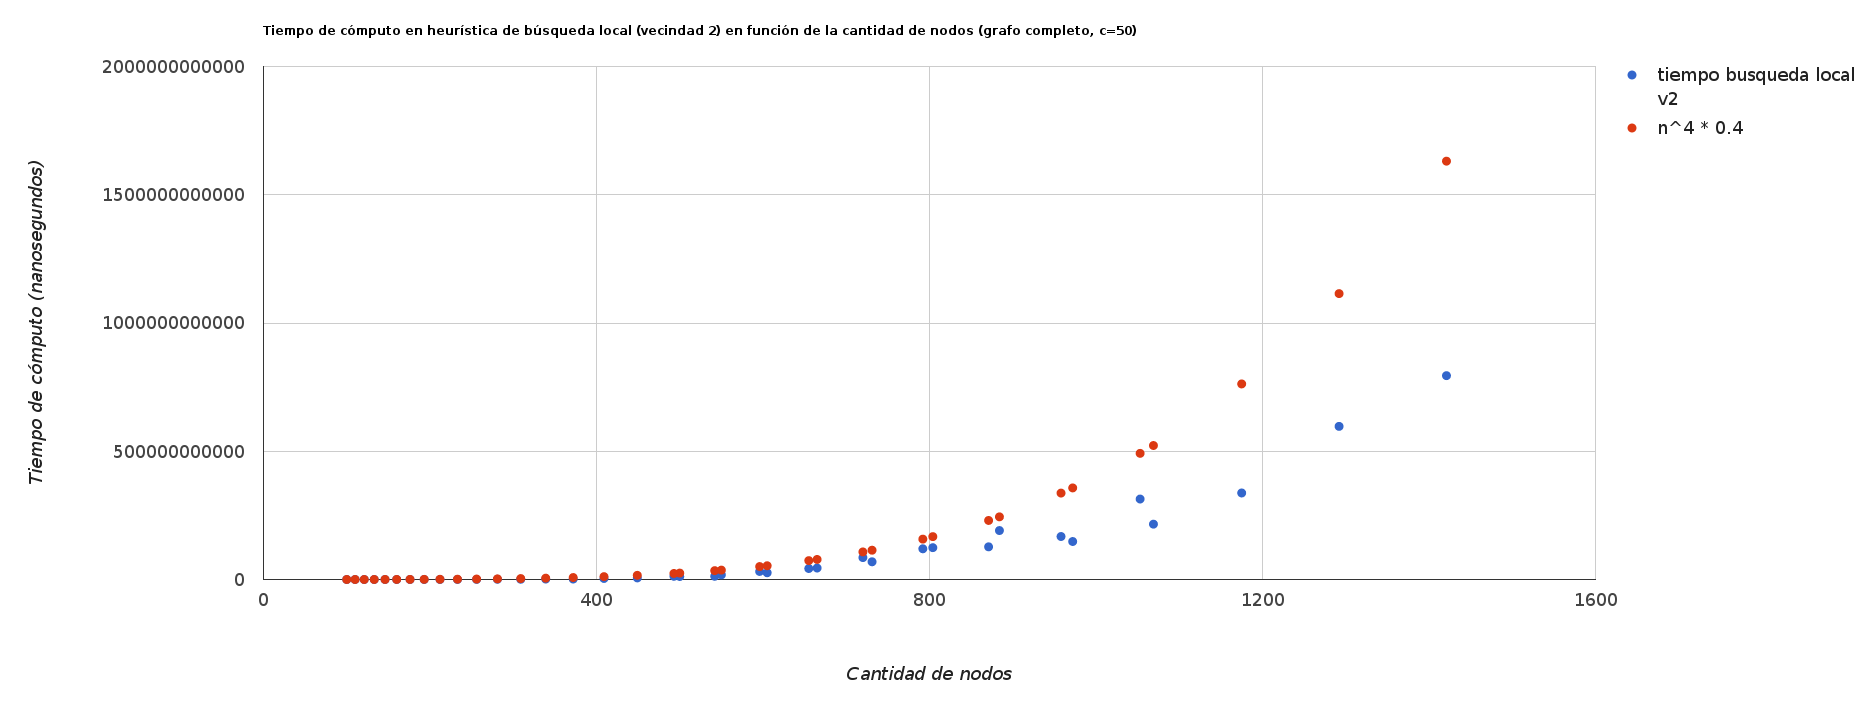
\includegraphics[width=18cm]{imagenes/Ej4/TvsNodosV2.png}
	\caption{Tiempos de cómputo en vecindad 2 en función de la cantidad de nodos.}
	\label{nodosEj4-v2}
 \end{figure}
 
También analizamos cómo variaba el tiempo de cómputo en función de la cantidad total de aristas. En la figura \ref{aristasEj4-Comp} se ve claramente que la vecindad 2 tiene una complejidad de un órden mayor que la de la vecindad 1.




\begin{figure}[H]
	\centering
 	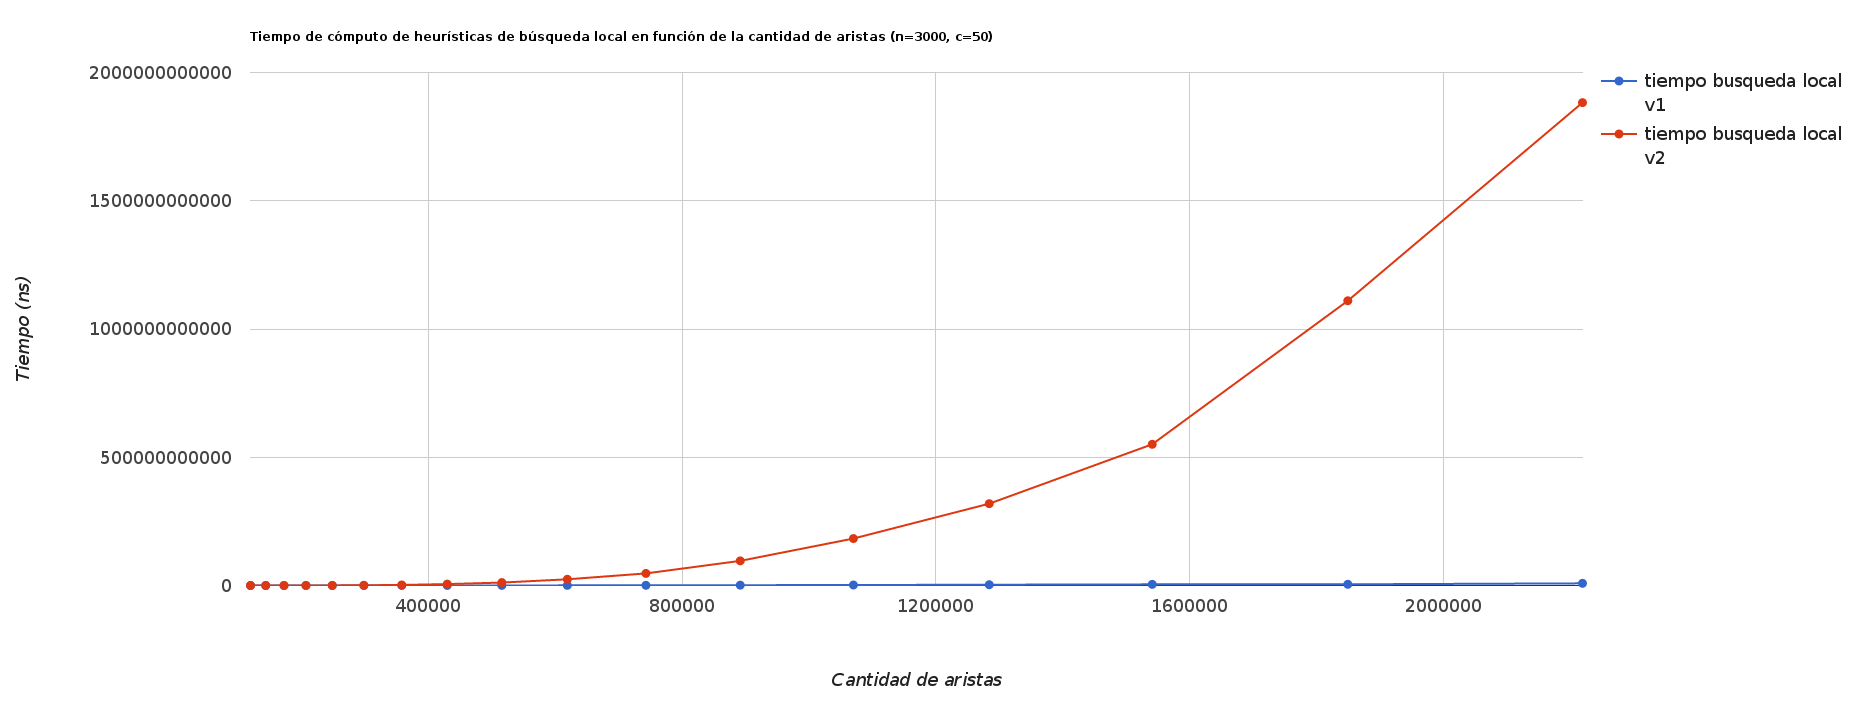
\includegraphics[width=18cm]{imagenes/Ej4/TvsAristasComp.png}
	\caption{Tiempos de cómputo en búsqueda local en función de la cantidad de aristas.}
	\label{aristasEj4-Comp}
 \end{figure}

\begin{figure}[H]
	\centering
 	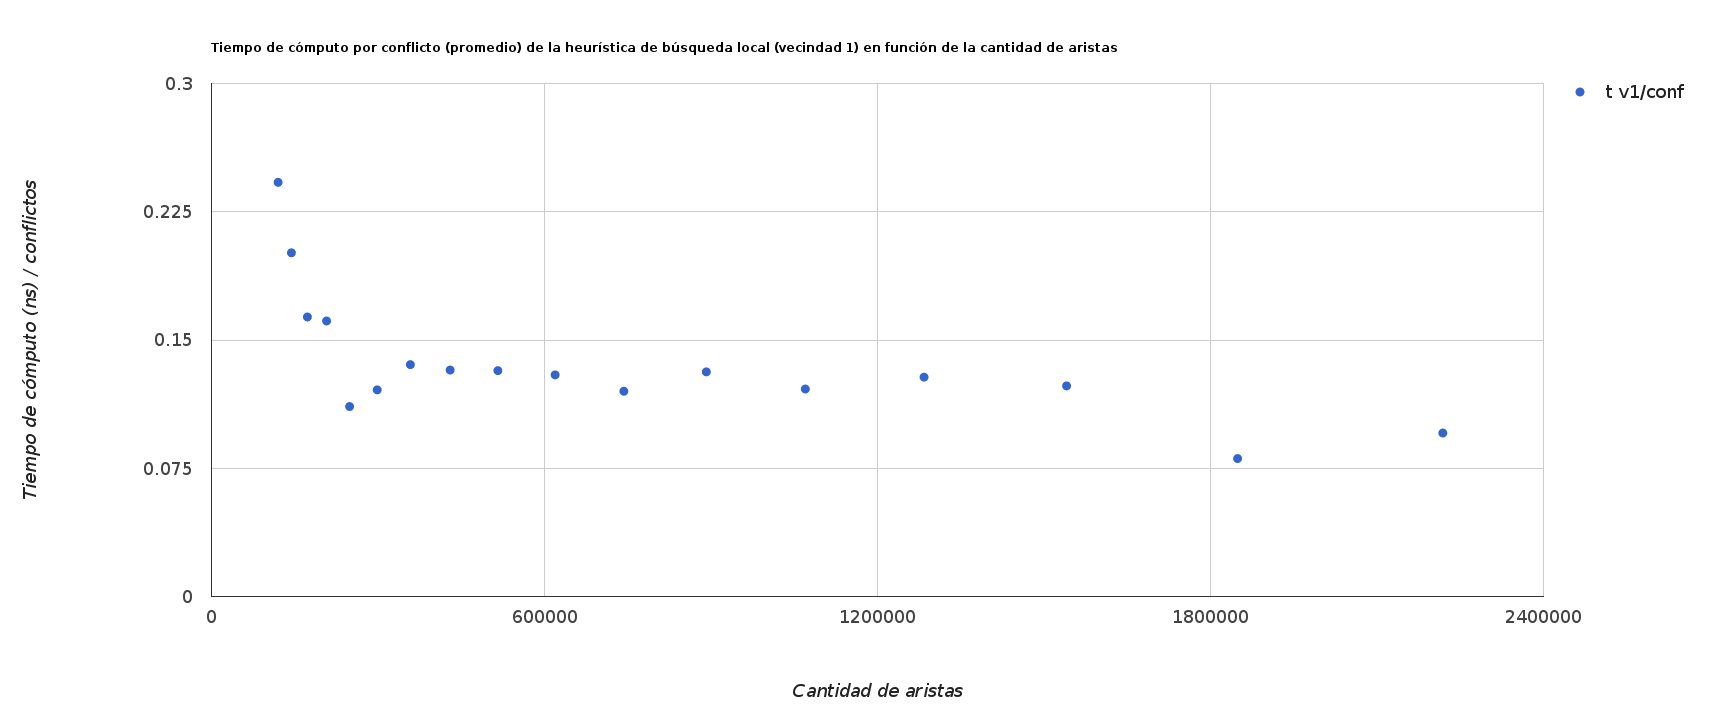
\includegraphics[width=18cm]{imagenes/Ej4/tiempoPorConflictovsAristasV1.png}
	\caption{Tiempos de cómputo por conflicto (promedio) con vecindad 1 en función de la cantidad de aristas.}
	\label{aristasEj4-V1}
 \end{figure}
 
 \begin{figure}[H]
	\centering
 	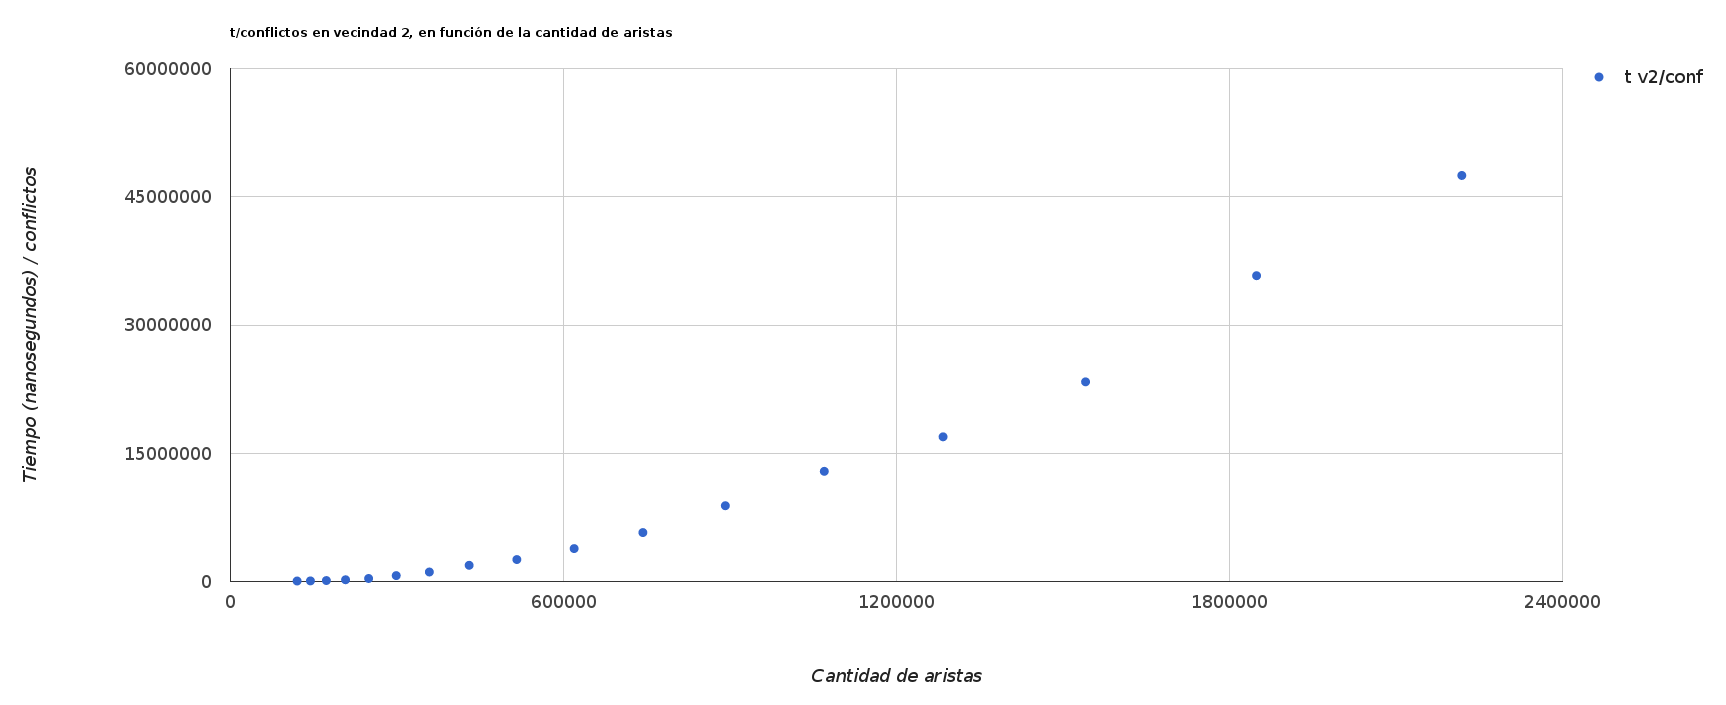
\includegraphics[width=18cm]{imagenes/Ej4/tiempoPorConflictovsAristasV2.png}
	\caption{Tiempos de cómputo por conflicto (promedio) con vecindad 2 en función de la cantidad de aristas.}
	\label{aristasEj4-V2}
 \end{figure}
 
 Las figuras \ref{aristasEj4-V1} y \ref{aristasEj4-V2} las realizamos para ver la correlación entre el tiempo de cómputo y la cantidad de conflictos inicial con la que inicia la ejecución del algoritmo. En la vecindad 1 se ve una relación lineal entre la cantidad de conflictos y el tiempo de ejecución (manteniendo la cantidad de nodos y de colores constante). En la vecindad 2 no vemos esto tan claro. Quisimos hacer un análisis más profundo pero los tiempos de ejecución son bastante prolongados y no fue posible realizar el análisis en un tiempo razonable.
 

 
 Y en función de la cantidad total de colores.
 
  \begin{figure}[H]
	\centering
 	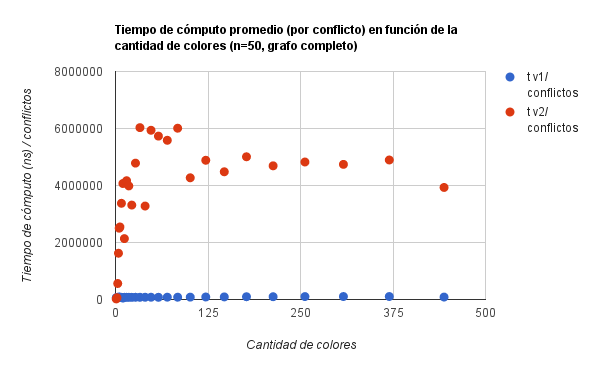
\includegraphics[width=18cm]{imagenes/Ej4/TvsColores.png}
	\caption{Tiempos de cómputo en búsqueda local en función de la cantidad de colores.}
	\label{coloresEj4-2}
 \end{figure}
 
 También hicimos una comparación entre la cantidad de conflictos que se resuelven con las distintas heurísticas.
 



 
 
 
 \subsubsection{Cantidad de conflictos resueltos}
 
   \begin{figure}[H]
	\centering
 	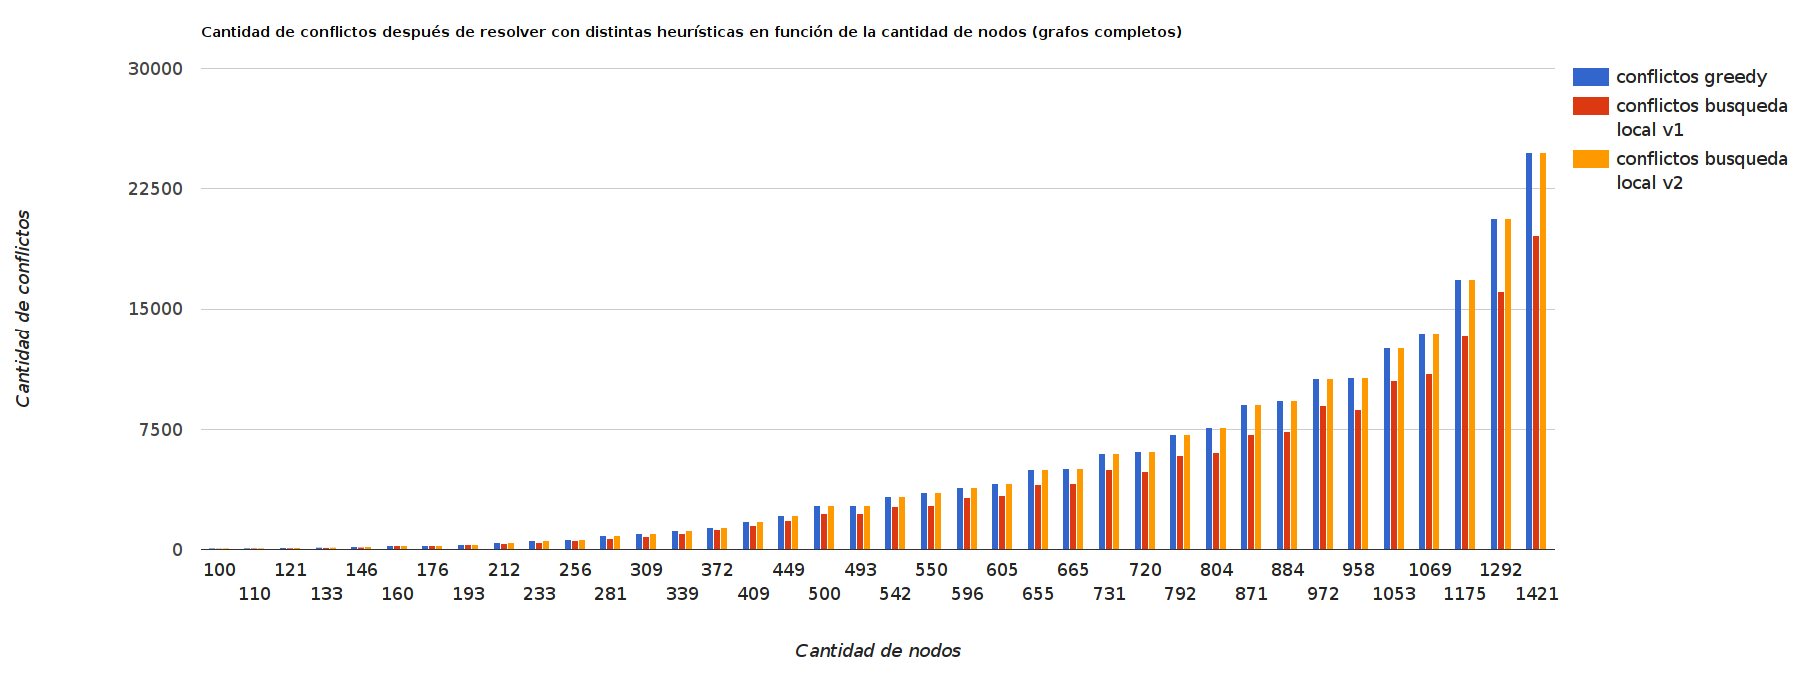
\includegraphics[width=18cm]{imagenes/Ej4/conflictosVsNodos.png}
	\caption{Cantidad de conflictos en el grafo luego de resolver usando distintas heurísticas/vecindades.}
	\label{conflictosEj4}
 \end{figure}
 
 \begin{figure}[H]
	\centering
 	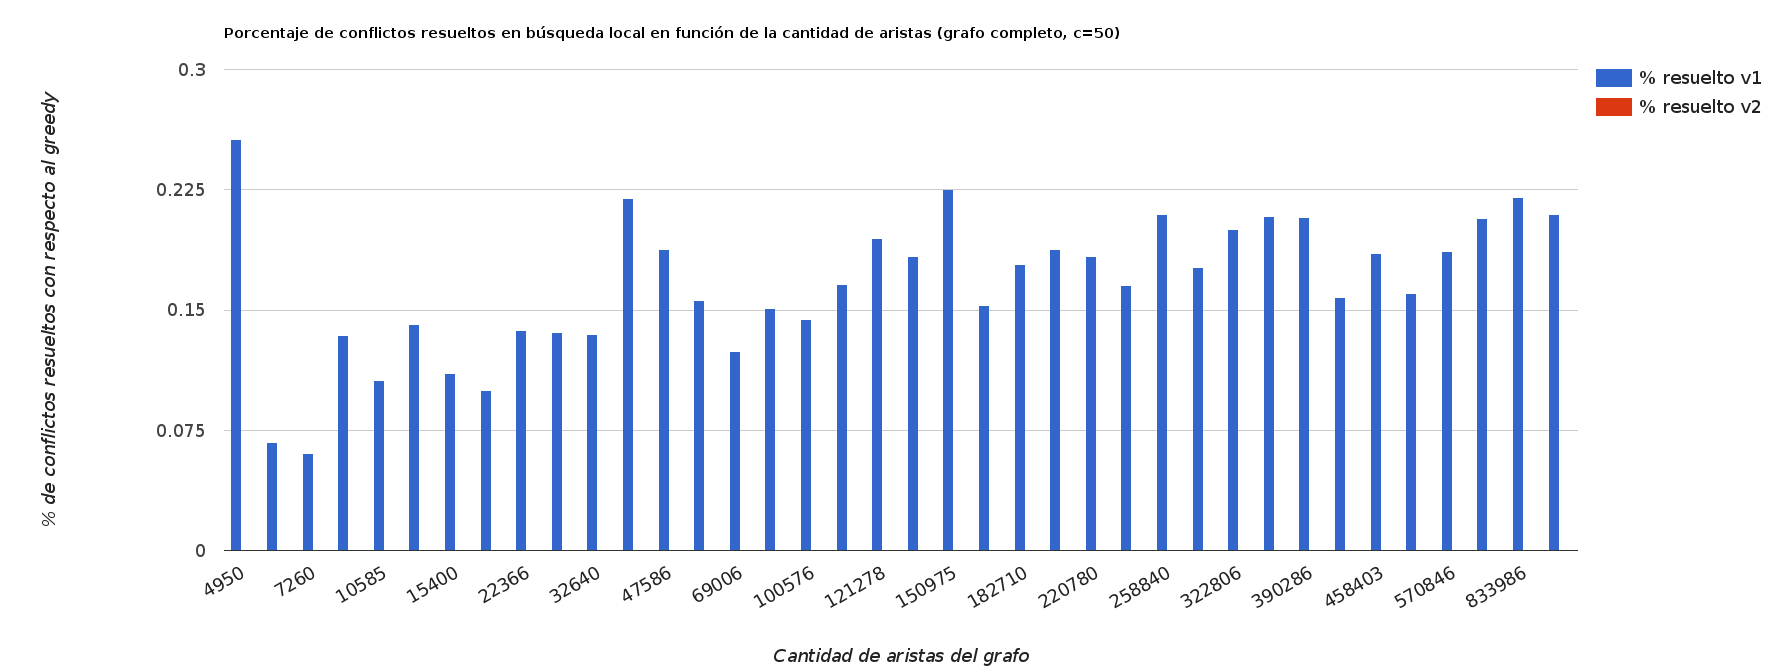
\includegraphics[width=18cm]{imagenes/Ej4/porcentajeConflictosVsAristas.png}
	\caption{Porcentaje de conflictos resueltos por cada vecindad en función de la cantidad de aristas.}
	\label{conflictosEj4-porcentaje}
 \end{figure}
 
 
  \begin{figure}[H]
	\centering
 	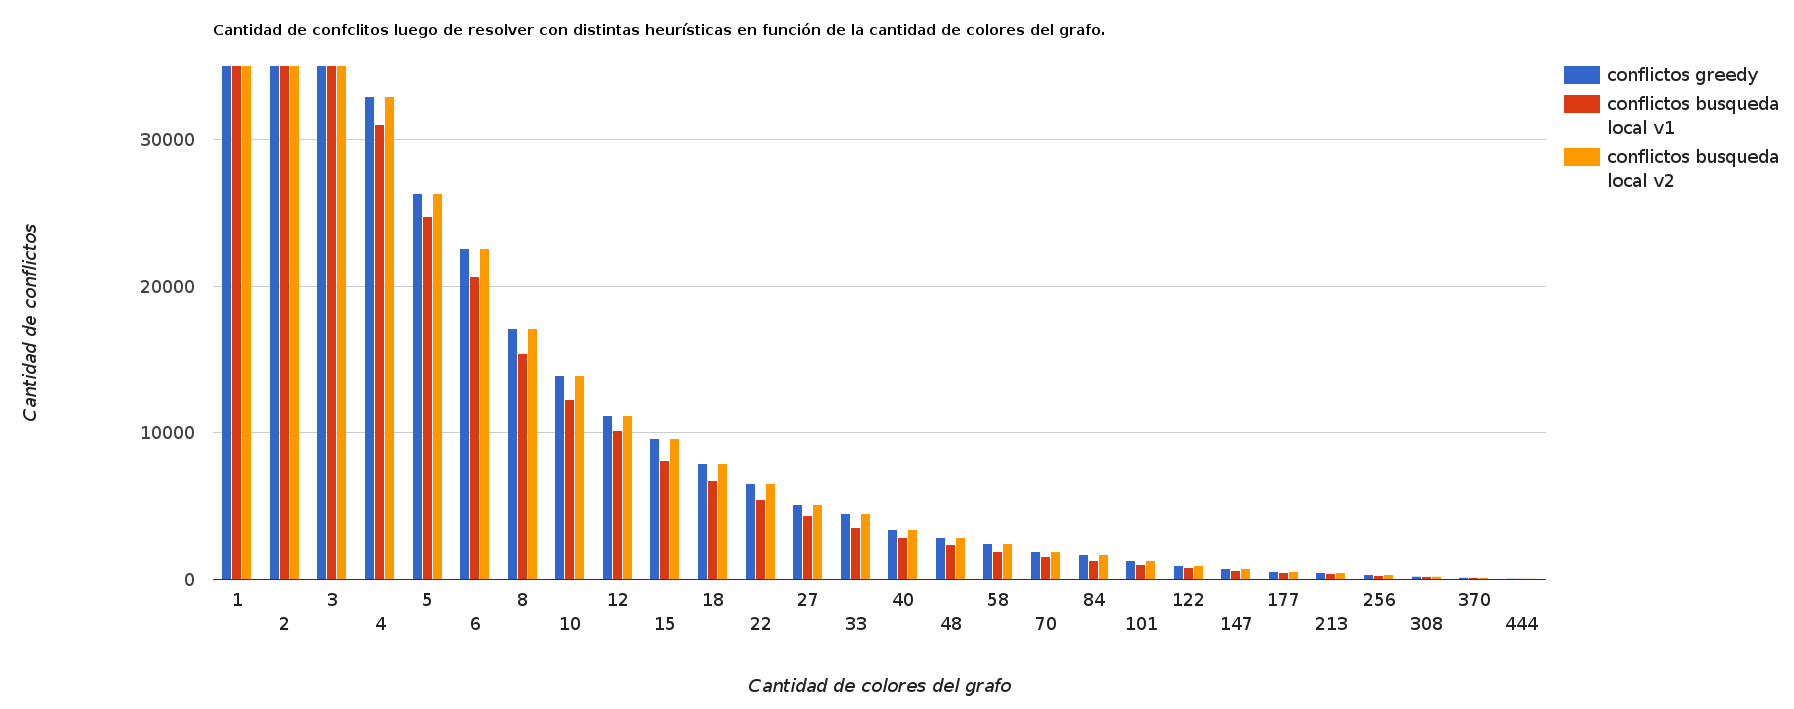
\includegraphics[width=18cm]{imagenes/Ej4/conflictosVsColores.png}
	\caption{Porcentaje de conflictos resueltos por cada vecindad en función de la cantidad de colores.}
	\label{conflictosEj4-porcentaje}
 \end{figure}
 
 
 La vecindad 2 no mostró buenos resultados. Por eso decidimos utilizar la vecindad 1.
% !TEX root = ./informe.tex
\newpage
\section{Apéndice: Código fuente}

A continuación se incluyen las partes más relevantes del código.\\

\subsection{2-List Coloring}

La clase lector se encarga de leer la entrada y transforla en un grafo. Como en los test de complejidad es importante no medir el tiempo que se tarda en cargar el archivo en memoria, el Lector posee funciones para cargar la información sin procesar.
\lstinputlisting[name=pp, numbers=left, frame=lines, firstline=105, lastline=161]{../ej1/src/Lector.java}
Los metodos que construyen el coloreo se encuentran en Calculador_de_Coloracion_Ej1 \\
\lstinputlisting[name=gr, numbers=left, frame=lines, firstline=114, lastline=183]{../ej1/src/Calculador\string_de\string_Coloracion\string_Ej1.java}


\newpage

\subsection{List Coloring}

La clase \emph{Main.java} se encarga de hacer el backtracking para recorrer todos los nodos fijando de a dos colores:
\lstinputlisting[name=main, numbers=left, frame=lines, firstline=39, lastline=52]{../ej2/src/Main.java}
\lstinputlisting[name=main, numbers=left, frame=lines, firstline=73, lastline=104]{../ej2/src/Main.java}
La clase \emph{LectorEj2.java} se encarga de leer el input y transformarlo en dos grafos, uno que contiene todos los colores y el otro que tiene un máximo de dos colores para poder pasarselo como parámetro a \emph{2ListColoring}. También hace el preprocesamiento de los datos para la última poda.
\lstinputlisting[name=lec, numbers=left, frame=lines, firstline=57, lastline=110]{../ej2/src/LectorEj2.java}
\lstinputlisting[name=lec, numbers=left, frame=lines, firstline=112, lastline=142]{../ej2/src/LectorEj2.java}
La clase \emph{Nodo_Coloreable_ej2} es muy similar a la clase \emph{Nodo_Coloreable_ej1}, lo único que cambia es que esta acepta una lista de mas de dos colores.
\lstinputlisting[name=nc, numbers=left, frame=lines, firstline=12, lastline=16]{../ej2/src/Nodo\string_Coloreable\string_ej2.java}


\subsection{Heurística Constructiva Golosa}

La clase \emph{Lector.java} se encarga de tomar los datos del archivo de entrada y procesarlos para construir el grafo mediante el método \textit{MakeGraph()}:\\

\begin{lstlisting}
	public Grafo MakeGraph() throws IOException
	{
		Grafo grafo = new Grafo();
		int[] nodosAristasColores = Ej3Utils.ToIntegerArray(this.getArchivo().readLine().split(" "));
		grafo.cantidadDeNodos = nodosAristasColores[0];
		grafo.setCantidadDeAristas(nodosAristasColores[1]);
		grafo.setCantidadDeColores(nodosAristasColores[2]);

		try { grafo.setNodos(this.ObtenerListaDeNodos(grafo.cantidadDeNodos, grafo.getCantidadDeColores()));}
		catch (IOException e) { System.out.println("Se produjo un error al generar los nodos del grafo.");}
		boolean[][] matrizDeAdyacencia = GenerarMatrizDeAdyacencia(grafo.getCantidadDeNodos(), grafo.getCantidadDeAristas(), false);
		grafo.setListaDeAdyacencia(Ej3Utils.matrizDeAdyacenciaToListDeAdyacencia(matrizDeAdyacencia, grafo.getNodos()));

		return grafo;
	}

\end{lstlisting}


La clase \emph{Grafo.java} contiene el método \textit{MakeRainbow()} que colorea el grafo con la heurística \newline propuesta: \\

\begin{lstlisting}
	public void MakeRainbow() // O(n^2*c*log(n))
	{
		int nodosPintados = 0;
		LinkedList<Nodo> colaNodos = new LinkedList<Nodo>();

		while(nodosPintados < this.cantidadDeNodos)
		{
			colaNodos.add(PicANode(this)); //O(1)

			while (!colaNodos.isEmpty()) //O(n)
			{
				Nodo nodoActual = colaNodos.removeFirst(); //O(1)

				if (!nodoActual.isVisitado())
				{
					colaNodos.addAll(this.getVecinosDe(nodoActual)); //O(n)
					LinkedList<Integer> coloresRestantes = nodoActual.getColoresRestantes(); //O(1)
					PintarNodo(nodoActual, coloresRestantes, this); //O(c*n*log(n))
					nodosPintados ++;
					nodoActual.setVisitado(true); //O(1)
				}
			}
		}
	}

	private static Nodo PicANode(Grafo grafo)
	{
		Nodo next = new Nodo();
		for(Nodo nodo : grafo.getNodos())
		{
			if (!nodo.isVisitado())
			{
				next = nodo;
				break;
			}
		}
		return next;
	}

	private static void PintarNodo(Nodo nodoActual, LinkedList<Integer> coloresRestantes, Grafo grafo) //O(c*n*log(n))
	{
		int colorAPintar = CalcularColorMenosPerjudicial(nodoActual, grafo); //O(c*n*log(n))
		nodoActual.setColor(colorAPintar);
	}

	private static int CalcularColorMenosPerjudicial(Nodo nodoActual, Grafo grafo) //O(c*n*log(n))
	{
		Double pesoColor = 1.0;
		int colorAPintar = -1;
		for (int color : nodoActual.getColoresRestantes()) //O(c)
		{
			Double peso = CalcularPeso(color, grafo.getVecinosDe(nodoActual)); //O(nlog(n))
			if (peso <= pesoColor)
			{
				pesoColor = peso;
				colorAPintar = color;
			}
		}
		return colorAPintar;
	}


	private static Double CalcularPeso(int color, List<Nodo> vecinos)
	{
		ArrayList<Double> pesos = new ArrayList<Double>();
		for (Nodo nodo : vecinos) //O(n)
		{
			if (nodo.LeImportaQueSuVecinoSePinteDelColor(color)) //O(1)
					pesos.add(nodo.PeligroDePintarUnVecinoDelColor(color));//O(1)(amortizado)

		}
		Collections.sort(pesos); //O(nlog(n))
		Double pesoTotal = 0.0;
		for (int k = 0; k < pesos.size(); k++) //O(n)
			pesoTotal += pesos.get(k)/(k+2); //O(1)

		return pesoTotal;
	}

\end{lstlisting}


\subsection{Búsqueda Local}

\subsubsection{Vecindad 1}

%\lstinputlisting[name=main, numbers=left, frame=lines, firstline=39, lastline=52]{../ej4/src/GrafoEj4.java}



\end{document}

